\chapter{Prototype simulations and design}
\chaptermark{Prototype simulations and design}
\cleardoublepage
\minitoc
\section{Introduction}
\begin{refsection}
  \label{ch3:Introduction}
  In the previous chapter, we described different ways to measure a transverse beam profile. At \acrshort{ess}, both invasive and non-invasive profilers will be installed along the accelerator. The beam profile will be also recorded on the target location and upstream of the beam dump \cite{shea2013}. The interceptive measurements are mainly done with wire scanners (\acrshort{ws}). These devices cannot handle the huge beam peek power of \acrshort{ess} at nominal conditions (125MW), and will be only used at low beam duty cycle \cite{Cheymol2013}. Therefore, Non invasive Profile Monitors, or \acrshort{npm}, will take over for higher beam power. The \acrshort{npm}s refer to two types of devices depending on the detection principle. Ionization Profile Monitors (\acrshort{ipm}) will be implemented exclusively in the cryogenic part of the accelerator whereas Fluorescence Profile Monitors (\acrshort{fpm}) are foreseen for all the remaining parts of the linac \cite{Thomas2016}. Our team is in charge of the design and the production of ten \acrshort{ipm}s. More information about the whole beam diagnostic framework at \acrshort{ess} is available in these documents \cite{Peggs2013,Shea:IBIC2017-MO2AB2}.

  The present chapter is dedicated to the studies and simulations performed in order to design the future \acrshort{ipm}s for \acrshort{ess}. Indeed, the ESS conditions are challenging and the feasibility of IPMs is not confident. In the following, we would like to introduce and define the goals and requirements of this project, and why \acrshort{ipm} has been foreseen. Then, several feasibility key-points will described and explained including expected counting rates, profile distortion effects and readout simulations.

  % TODO: introduire le GONOGO
  % Then feasibility keypoints were studied like counting rate, space charge and field uniformity and will described and explain in the next sections.
  \section{ESS requirements}
  This section is not the most exciting one but it still interesting to underline the different requirements and specifications that our devices should match. \acrshort{ess} has defined requirements for the whole machine, and they are organized on different levels starting from installation to subsystems. Every subsystem must meet their specification levels. In the case of the \acrshort{npm} system, the most importants are defined in the level 4 (beam instrument) and level 5 (non invasive profile monitor) requirements:
  %TODO: Reformuler
  \begin{itemize}
    \item The transverse beam profile shall be measured with a total measurement error in the RMS extension of the beam of less than $\pm10\,\%$.
    \item A spatial resolution of \(\leq\ 0.05\,\mathrm{mm}\) shall be achieved.
    \item The devices must perform the measurements and report the relevant data at a repetition rate of \(14\,\mathrm{Hz}\).
    \item The detectors shall have a dynamic range of $1000$.
  \end{itemize}

  Each cold \acrshort{npm} consists of a consecutive pair of \acrshort{ipm}s, each \acrshort{ipm} measuring a transverse projection. The pair is plugged in a specific vacuum vessel: the Linac Warm Unit (LWU). The design of the \acrshort{lwu} has been mostly frozen just few weeks after the kickoff meeting of cold \acrshort{npm} project (may 2016). Two \acrshort{lwu} designs have to be considered for the \acrshort{ipm}s: one for the Spoke section and another one for the elliptical section which differs slightly. A pair of wire scanners is also mounted on the \acrshort{lwu}. The \acrshort{ipm}s should not overlap on the \acrshort{ws} area, even if the wire scanners work only at low duty cycle whereas the \acrshort{ipm}s operate at higher duty cycle. The minimal pipe radius is respectively \(50\,\mathrm{mm}\) and \(25\,\mathrm{mm}\) for the Elliptical and the Spoke \acrshort{lwu}. We designed our detector to match with all the previous mechanical specifications.

  \begin{figure}[ht]
	% Changer l'image car pas à jours.
	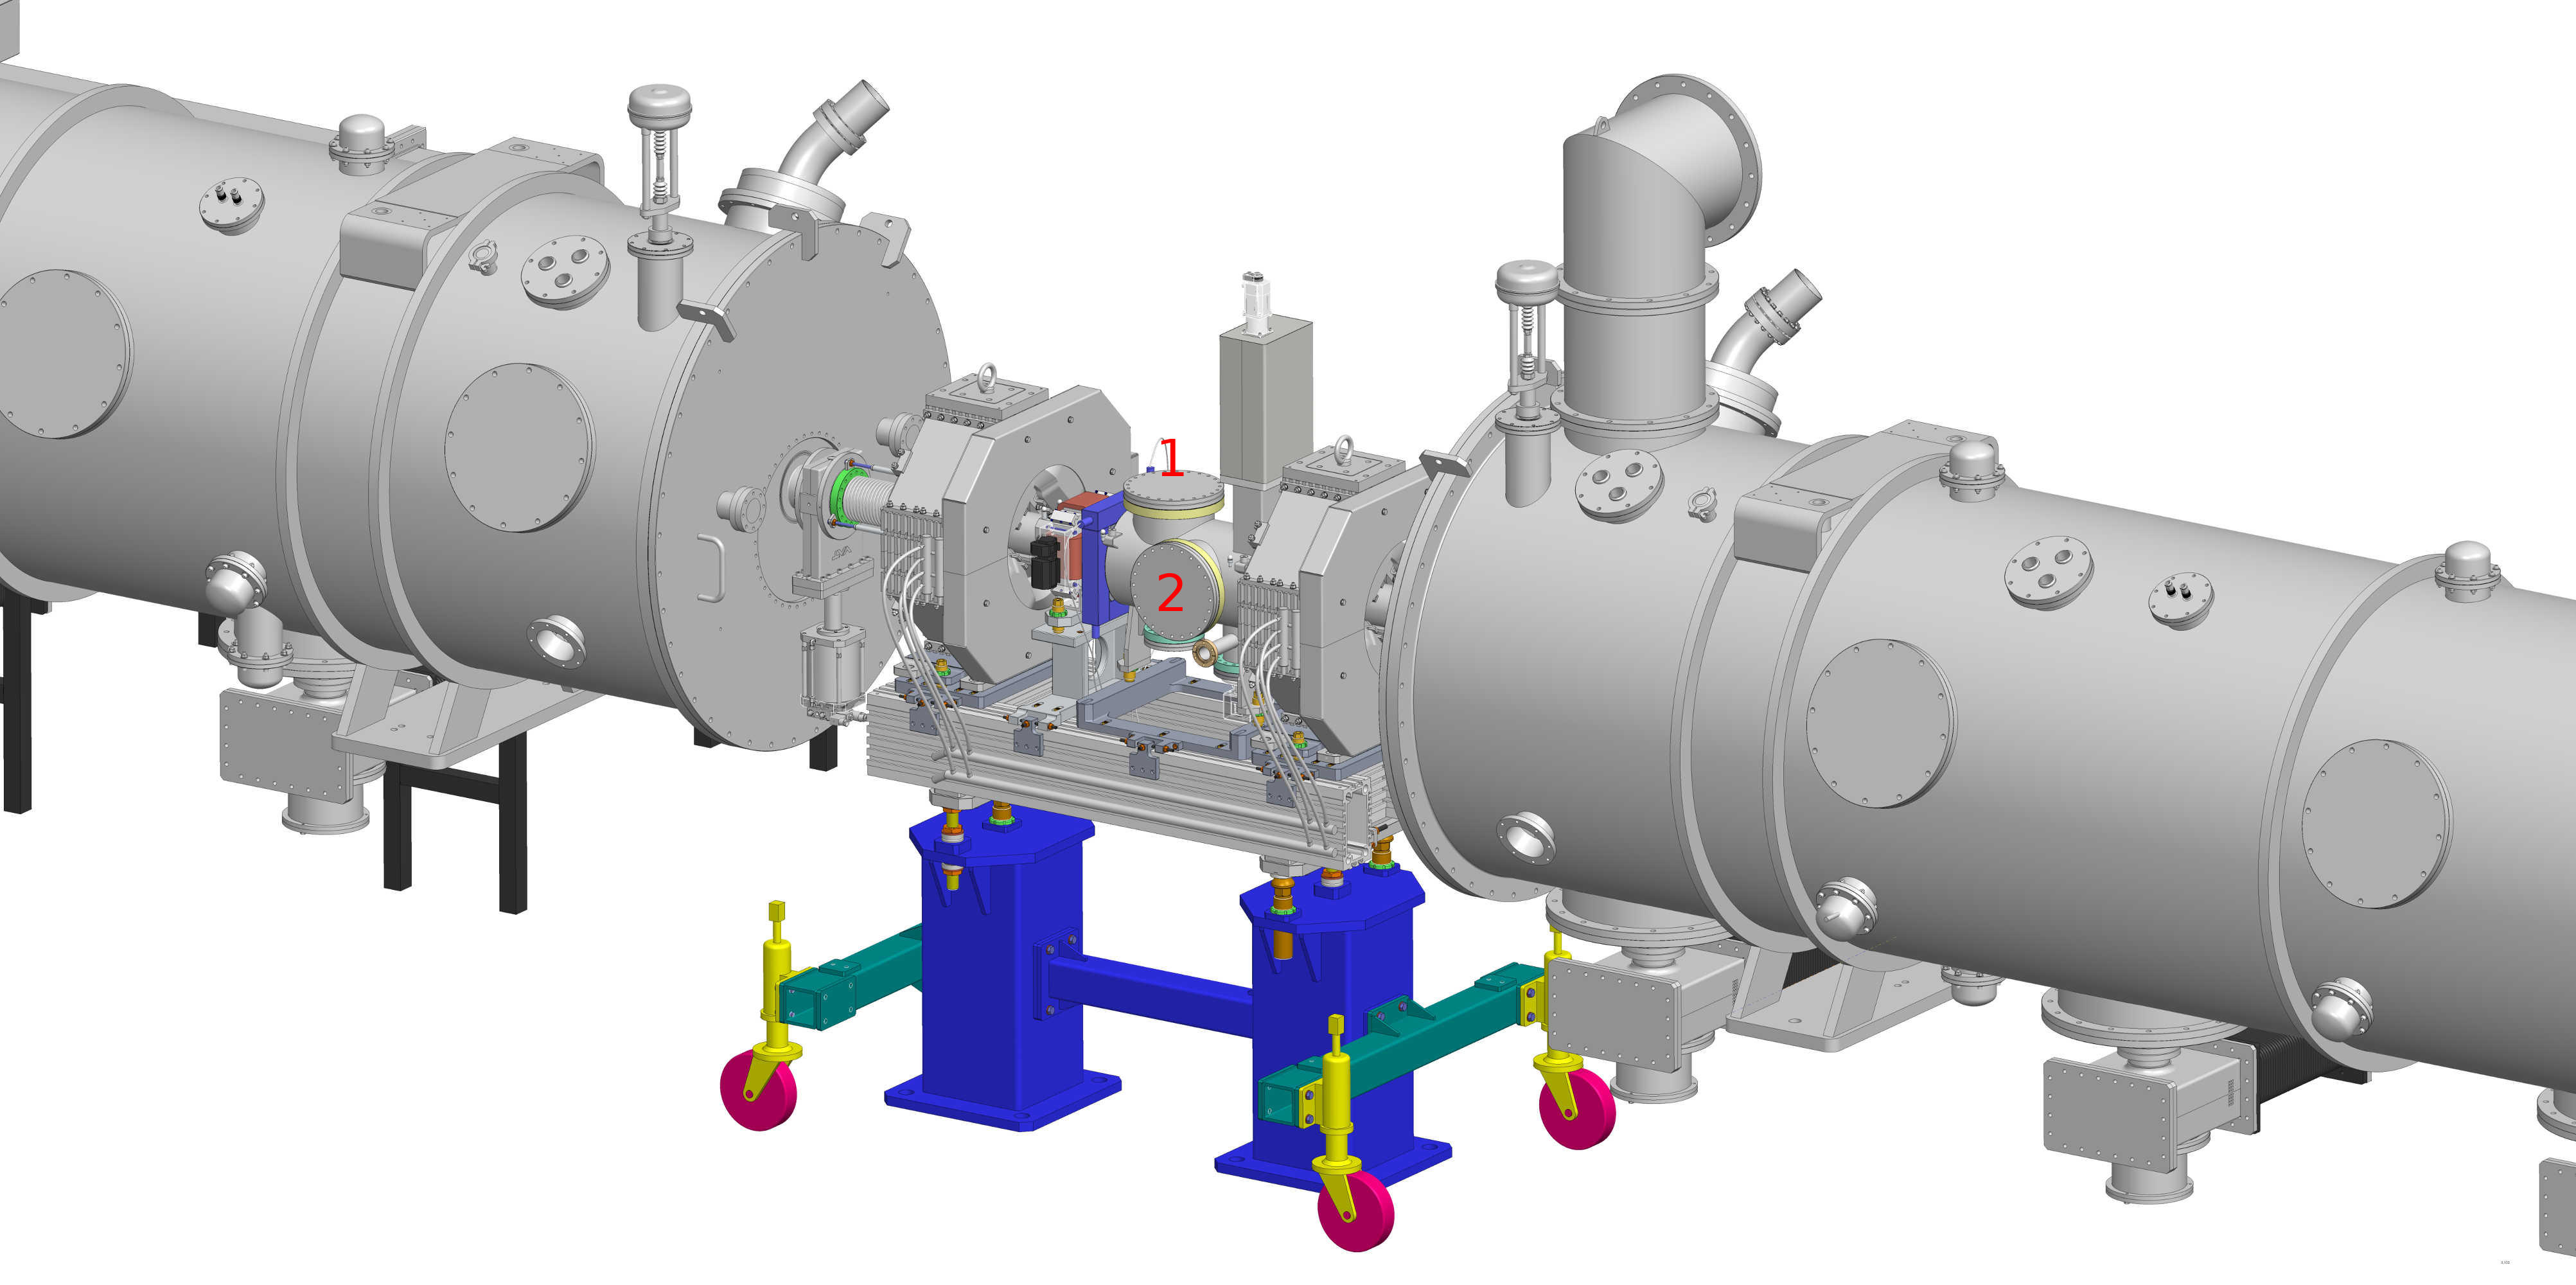
\includegraphics[width=\textwidth]{03_Prototype/figures/fig016_LWU_Cryo3.jpeg}
	\caption[The LWU vessel located between two quadrupole magnets and two cryomodules]{The LWU vessel located between two quadrupole magnets and two cryomodules. The IPMs will be mounted on the CF 200 flanges 1 and 2.}
	\label{chap3:LWU_Cryo}
\end{figure}


  The \acrshort{ipm} will be located between two cryomodules in the accelerator cold. The \acrshort{lwu} vessels itself are not cooled down however the superconducting cavities are closeby. The use of superconducting cavities imposes a high vacuum and a clean environment. Indeed, a too high pressure or a contamination may damage the cavities. An operating pressure of \(10^{-9}\,\mathrm{mbar}\) is foreseen but the vacuum level may be even lower during the operation. However, the safety valves will be closed if the vacuum reach \(10^{-7}\,\mathrm{mbar}\). Hence, our \acrshort{ipm} design must be compliant with a high vacuum level and particle-free environment. Fig. \ref{chap3:LWU_Cryo} shows the \acrshort{lwu} vessel in between two cryomodules. One can see the two \acrshort{cf} 200 flanges and the two rectangular \acrshort{cf} flanges for the wire scanners.

  \section{IPM simulations overview}

  \begin{wrapfigure}{r}{0.5\textwidth}
	\centering
	\begin{tikzpicture}%[scale=1.3]
		% Variables
		% Ipm
		\pgfmathsetmacro{\LIPM}{1.8};
		\pgfmathsetmacro{\HIPM}{1.8};
		\pgfmathsetmacro{\TIPM}{0.1};
		% Deg
		\pgfmathsetmacro{\LDEG}{0.1};
		\pgfmathsetmacro{\HDEG}{0.3};
		\pgfmathsetmacro{\NDEG}{6};
		\pgfmathsetmacro{\SDEG}{1.5};
		\pgfmathsetmacro{\SPAND}{(2*\SDEG - \HDEG)/\NDEG}

		\draw[] (\LIPM,0) node[right,align=left] {Field\\correctors\\or\\degraders};


		% Beam
		\draw[fill=blue!30] (0,0) circle (0.4) node[left,xshift = -0.3cm] {Beam};
		% Cage
		\draw (0,0) (-\LIPM,\HIPM)rectangle(\LIPM,\HIPM+\TIPM) node[above] {Anode};
		\draw (0,0) (-\LIPM,-\HIPM)rectangle(\LIPM,-\HIPM-\TIPM) node[below] {Cathode};
		\draw[fill=red!50] (-\LIPM/2,-\HIPM) rectangle(\LIPM/2,-\HIPM-\TIPM) node[midway,below] {Readout};
		% Ionized particle
		\draw[blue, dashed,->] (0.1,0.8)--(0.1,\LIPM);
		\draw[blue,fill=blue] (0.1,0.8) circle [radius=1mm] node[] {\tiny\color{white}{$-$}};

		\draw[red, dashed,->] (0.16,-1)--(0.16,-\LIPM);
		\draw[red,fill=red] (0.16,-1) circle [radius=1mm] node[] {\tiny\color{white}{$+$}};

		\draw[blue,dashed,->] (-0.1,0.1)--(-0.1,\LIPM);
		\draw[blue,fill=blue] (-0.1,0.1) circle [radius=1mm] node[] {\tiny\color{white}{$-$}};

		\draw[red,dashed,->] (-0.1,-0.1)--(-0.1,-\LIPM);
		\draw[red,fill=red] (-0.1,-0.1) circle [radius=1mm] node[] {\tiny\color{white}{$+$}};

		%Field
		\draw[->] (-1.2,1.5)--(-1.2,0.6) node [midway,right]{$\vec{E}$};
		% Degradors
		\foreach \x in {0,...,\NDEG}{
				\draw (0,0) (-\LIPM,\x*\SPAND - \SDEG) rectangle (-\LIPM+\LDEG,\x*\SPAND+\HDEG-\SDEG);
				\draw (0,0) (\LIPM,\x*\SPAND - \SDEG) rectangle (\LIPM-\LDEG,\x*\SPAND+ \HDEG-\SDEG);}


		%Profile
		\begin{axis}[every axis plot post/.append style={
						mark=none,domain=-3:3,samples=50,smooth},
				clip=false,
				axis y line=none,
				axis x line*=bottom,
				ymin=0,
				ymax=1,
				xtick=\empty,
				width=4cm,
				height=3cm,
				scale only axis,
				xshift=-2cm,
				yshift=-3.5cm
			]
			\addplot {\gauss{0}{0.3}{0.3}};
		\end{axis}

	\end{tikzpicture}
	\centering
	\caption[Visual explanation of how an IPM works]{Visual explanation of how an IPM works. The electric field between the electrodes can be reverted by inverting the polarity, making it possible to choose if detecting ions or electrons. Field correctors or degradors, left and right, improve the field uniformity.}
	\label{chap3:ipm_outline}
\end{wrapfigure}


  As explained in the previous chapter, Ionization Profile Monitor (\acrshort{ipm}) is a non-invasive detector that measures the transverse profile of a beam (\acrshort{npm}).
  The principle of operation is summarized in the Figure \ref{chap3:ipm_outline} and in the three main steps:
  \begin{enumerate}
    \item Protons from beam pass through the vacuum, inducing ionizations on the residual gas molecules: electron/ion pairs are created.
    \item Inside the \acrshort{ipm}, a strong electric field drives electrons or ions towards a segmented readout system.
    \item The profile is reconstructed in one transverse direction. For a complete profile, a pair of \acrshort{ipm}s, rotated by $90\textdegree{}$ to each other, is mandatory.
  \end{enumerate}

  Unfortunately, there is not simulation framework that allows a full simulation of an \acrshort{ipm}. Each simulation step requires unique tools. In fact, most of the work consist of linking each simulation step together. The simulation can be split in three main categories, the same as the detector behaviour explained just above. In this chapter, we describe in the same order all the simulations and approximations that has helped us to design our detector.

  Firstly, the primary number of particle created by the proton beam should be evaluated, and it must be sufficient in order to reconstruct a beam profile. However, this does not guaranteed that the primary particles reach the readout plane. Thus, it is necessary to perform some electromagnetic simulations. Indeed, primary particle are sensitive to the non uniformities of the extraction field and to space charge effects induced by the beam. These effects may disturb the profile measurements or reduce the number of primary particles. Therefore, they should be quantified. Lastly, the signal creation in the readout device should be evaluated with respect to previous simulations. The response of the readout mainly depends on its type.

  \section{Particle through matter}
  The interactions of particles with matter are an important aspect of particle detection \cite{Knoll2010,Leo1994}. A particle will lose energy when it passes through a medium. The physical process behind the energy transfer mainly depends on the characteristics of the particle and the medium. These topics have been studied and improved over the last century. It often combines complicated theoretical laws with approximations or empirical models. This topic is very wide, hence in the following only the pertinent information for this study will be described.

  As explained before, the \acrshort{ipm}s rely on the by-product collection of the ionized residuals gas. The number of ionized particles gives the signal strength which has to be compliant to the readout sensitivity. Therefore, we need to know how many particles are created by the beam itself along the residual gas enclosed in the accelerator beam pipe. Then we should understand how theses secondary particles create signal in the sensitive part of our \acrshort{ipm}.


  \subsection{Interaction of charged particles with matter}
  For heavy charged particles, the main interaction is due to electromagnetic interactions of the incident particle with the orbiting electrons of the medium. A particle is considered heavy if its mass is much higher than the mass of an electron. The incident particle will transfer a small amount of its energy to an electron of the medium at each electronic collision. In 1930 Bethe proposed an equation that describes the mean rate of energy losses per distance of a heavy charged particle \cite[]{Bethe1930}. The so-called Bethe equation derives from the coulomb interactions. This equation has been improved over the years \cite{Bloch1933,Fermi1940,Fano1963}. The expression of the linear stopping power for heavy charged particle is defined by the following equation \cite[p. 446]{Tanabashi2018}:
  \begin{equation}
    - \bigg \langle \frac{dE}{dx} \bigg \rangle =K \rho \frac{Z}{A} \frac{z^{2}}{\beta^{2}} \left[\frac{1}{2} ln \left(\frac{2 m_{e} \beta^{2} \gamma^{2} T_{max}}{I^{2}} \right) - \beta^{2} - \frac{\delta(\beta \gamma)}{2} - \frac{C}{Z} \right]
  \end{equation}

  Where \(K\) is a constant factor defined by \(K=4 \pi N_{a} r_{e}^{2} m_{e} c^{2}\), \(r_{e}\) is the classical electron radius, \(m_{e}\) is the electron mass, \(N_{a}\) the Avogadro constant and c the speed of light in vacuum. For convenience, the stopping power is usually expressed in \(\mathrm{MeV/cm}\). In this case, \(K\) is equal to \(0.307075\).

  Terms in the Bethe equation can be dissociated in two groups. First, the incident particle related terms. The maximum transfer energy for one collision is given by the following equation:
  \begin{equation}
    T_{max} = \frac{2 m_{e} \beta^{2} \gamma^{2}}{1 + \frac{2 \gamma m_{e} }{M} + \left( \frac{m_{e}}{M} \right)^{2}}
  \end{equation}
  Where, \(M\) and \(m_{e}\) are respectively the incident particle and electron masses. The \(\beta\) and \(\gamma\) variables have their normal significance of the Lorentz factors.

  Finally, the terms related to the medium. \(Z\), \(A\) and \(\rho\) are respectively the atomic number, the mass number and the density of the given medium. In most of the cases the \(\frac{Z}{A}\) ratio is close to \(0.5\) except when a medium contains hydrogen. Sometime, the Bethe equation is given independently from the density.
  The mean excitation energy \(I\) is the only non trivial variable in the Bethe equation \cite{Berger1984,Berger1993}. The computation is quite complicated because it requires to measure  the oscillator strength for each material. Table \ref{chap3:WandI} gives the \(I\) value for common materials.

  Two correction factors are often used to improve the accuracy of the Bethe equation at low and high energies. The density effect \(\frac{\delta(\beta \gamma)}{2}\) corrects the effects at relativistic energies \cite{Sternheimer1984}. The shell correction \(\frac{C}{Z}\) improves the accuracy at low energies \cite{Bichsel2002}.

  \begin{figure}[!ht]
	\includesvg[width=\textwidth]{03_Prototype/figures/fig001_bethe_4}
	\caption[Typical mass stopping power plot a proton]{Typical mass stopping power plot for a proton. Here the mass stopping power is plotted for a proton in hydrogen and nitrogen. The calculation was done using the Bethe formula and has been cross-checked with the NIST PSTAR table which contains both computed and experimental values \cite{Seltzer1993}.}% The Bethe %equation gives correct results between \(0.2\ <\ \beta\gamma\ <\ 100\). %However at lower and higher energies the Bethe formula is no more reliable.}
	\label{chap3:bethe1}
\end{figure}


  Fig. \ref{chap3:bethe1} shows the mass stopping power of a proton in two different mediums. The blue region represents the energy range of protons in the cryogenic part of \acrshort{ess}, where \acrshort{ipm}s will be located. One can see that the minimum of energy loss is reached around \(2\,\mathrm{GeV}\).

  The Bethe model has been tested and improved with respect to experimental data \cite{Porter1990}. However, at very low or high energies the Bethe equation is no more usable. In these regions specific models are used to describe the energy loss in matter \cite{Ziegler1985, Allison1980}.

  The Bethe model is also not compatible with low mass particles like electrons and positrons. The Bethe formula must be modified for these particles \cite{Rieke1972}\cite[p. 452]{Tanabashi2018}. At low energies, electrons lose its energy by ionization like ions. Whereas at energies above few \(\mathrm{MeV}\), electrons also lose energy through bremsstrahlung radiation.

  \subsection{Electron ion pairs production}
  We just defined the mean energy loss rate of a charged particle per unit of distance. When a particle passes through a medium it may deposit its energy to an electron of the medium (atoms).
  If the energy is sufficient an ionization happens: an electron is ejected from the electronic shell leading to the creation of an ion and an electron. In case of molecule, the ionization process may be dissociative i.e. it may break the molecular bound. The cross section for dissociative ionization is far lower than the one for pure ionization \cite{Dimopoulou2004}.

  By introducing \(W\), the average energy to produce an ion/electron pair in a medium, it allows to estimate the number of ion/electron pairs created for a given detector length \cite[]{Weiss1955,Bichsel1979}.

  \begin{equation}
    N_{electrons}= \frac{\big \langle \frac{dE}{dx} \big \rangle}{W_{n}} \Delta x
  \end{equation}

  When an electron is ejected, it has a certain probability to ionize other atoms when its energy is high enough. These secondary electrons are called delta rays or delta electrons. This phenomena becomes rare and negligible when the medium has a very low density like in a vacuum system. The \(W\) parameter includes the delta ray electrons, hence the \(W\) value is biased for us since our detectors work at very low pressure \cite[p. 470]{Tanabashi2018}. Table \ref{chap3:WandI} gives, as an example, the \(W\) values for several materials.

  \begin{table}[ht]
	\centering
	\caption[Mean excitation energie, average energy to produce a pair and density values for severals mediums at Normal Temperature and Pressure (NTP)]
	{Mean excitation energie, average energy to produce a pair and density values for severals mediums at Normal Temperature and Pressure (NTP). Complete reviews of \(I\) and \(W\) values are available in \cite{Kamakura2006}\cite{Bichsel1979}.}
	\label{chap3:WandI}
	\begin{tabular}{llll}
		\toprule
		Gas        & \(I\) (\(\mathrm{eV}\)) & \(W\) (\(\mathrm{eV}\)) & \(\rho\) (\(\mathrm{kg/m^{3}}\)) \\
		\midrule
		\(H_{2}\)  & \(18.8\)       & \(36.43\)  &  \(0.0899\)  \\
		\(CO\)     & \(85.9\)       & \(34.5\)   &  \(1.165\)  \\
		\(CO_{2}\) & \(85.00\)      & \(34.21\)  &  \(1.842\)  \\
		\(N_{2}\)  & \(82.00\)      & \(36.39\)  &  \(1.165\)  \\
		\bottomrule
	\end{tabular}
\end{table}

  When the medium is a mixture of several compounds then it is necessary to calculate the mean stopping power for each of them weighted by their mass proportions:
  \begin{equation}
    N_{total}= \sum_{n= First}^{Last} N_{compound\ n}= \sum_{n= First}^{Last} w_{n} \frac{\big \langle \frac{dE}{dx}\left(\rho_{n},I_{n},A_{n},Z_{n}\right) \big \rangle}{W_{n}} \Delta x
  \end{equation}
  The calculation can be done for each single element or for each molecule in the compound.
  However, the second computation is preferable since the \(I\) values are in general higher for molecules \cite[p. 451]{Tanabashi2018}.

  \subsection{Calculation}

  Now that we have defined all the physics background, we should be able to estimate the number of primary particles that will be created in the \acrshort{ess} conditions. We tried two different approaches: naive computation of Bethe equation and simulations through a framework.

  The Bethe formula is easy to implement since it requires to know only the composition of the medium and the \(I\) value of each compound. The expected pressure in the cryogenic part at \acrshort{ess} is around \(10^{-9}\ mbar\), and the gas composition is given in Table \ref{chap3:ess_vacuum_gas}.

  \begin{table}[ht]
	\centering
	\caption[Expected residual vacuum gas in the cold part of ESS Linac, provided by ESS vacuum group]
	{Expected residual vacuum gas in the cold part of ESS Linac, provided by ESS vacuum group.}
	\label{chap3:ess_vacuum_gas}
	\begin{tabular}{llll}
		\toprule
		Gas        & Mass percentage (\(\%)\) & $p_{i}$ (\(\mathrm{mbar}\)) & $\rho_{i}$ $(\mathrm{g/cm^{3}}$) \\
		\midrule
		\(H_{2}\)  & \(79\)          & \(7.9 10^{-10}\)   & \(6.52\cdot
		10^{-17}\)                                                                \\
		\(CO\)     & \(10\)          & \(1.0 10^{-10}\)   & \(1.15\cdot
		10^{-16}\)                                                                \\
		\(CO_{2}\) & \(10\)          & \(1.0 10^{-10}\)   & \(1.8\cdot
		10^{-16}\)                                                                \\
		\(N_{2}\)  & \(1\)           & \(1 10^{-11}\)     & \(1.14\cdot
		10^{-17}\)                                                                \\
		\bottomrule
	\end{tabular}
\end{table}

  We assume that the residual gas follows the "perfect gas" law. We also assume that the linear density scaling of Bethe equation remains true in high vacuum \cite[p. 446]{egber2012}\cite{Ishimaru1995}. Hence, the partial pressure and the density for each gas is calculated with respect to the tabulated pressures. The primary signal is computed at \acrshort{ess} nominal conditions given in Table \ref{chap2:ess_charac}.

  Fig. \ref{chap3:ess_primary_particles} shows the number of electron ion pairs created for each gas species versus the \acrshort{ess} range of energies. The different \acrshort{ipm}s locations is marked by a blue line. One can see that the density has a strong influence on the primary signal. Although the hydrogen is the main species in term of proportion, its contribution to primary signal is close to the one from carbonate species. As explained just before, the \(W\) value may overestimate the number of pairs created due to secondary delta rays.

  \begin{figure}[!ht]
	\includesvg[width=\textwidth]{03_Prototype/figures/fig015_ess_primary_particle}
	\caption[Expected number of electron/ion pairs per centimeter at ESS nominal conditions according to Bethe equation]{Expected number of electron/ion pairs per centimeter at ESS nominal conditions according to Bethe equation. Each vertical line corresponds to an IPM location.}
	\label{chap3:ess_primary_particles}
\end{figure}


  We have also used Garfield++ software to compute the number of primary particles. This software is normally intended to the modelization gaseous detectors. It allows to simulate the creation of electron / ion pair due to the ionization of gas by an incident particle, the transport and the amplification of these electrons in the gas and the induced signal on a readout plane. In our case, we simulated only the pair creation in gas. For this step Garfield++ uses two programs internally:
  \begin{itemize}
    \item Magboltz: a Fortran routine that compute different properties of a gas mixture and the transport of electrons in this mixture \cite{Biagi1989}.
    \item Heed ++: a C ++ library that implements an ionization model based on the photoabsorption ionization (PAI) \cite{Allison1980,Smirnov2005}.
  \end{itemize}

  A dummy detector, a cube of ten centimeter, is implemented and filled with the same gas composition as the ESS residual gas. Then, we shoot protons into this detector. The information on the electrons created in gas is saved in a ROOT file and then processed. This is done for different proton energies and vacuum levels.

  \begin{table}[ht]%{r}{0.5\textwidth}
	\centering
	\caption[Comparison of expected number of electrons between calculation using Bethe equation and results from Garfield++.]
	{Comparison of expected number of electrons between calculation using Bethe equation and results from Garfield++}
	\label{chap3:GarfieldBethe}
	\begin{tabular}{llll}
		\toprule
		Energy    & \(N_{Bethe}\) & \(N_{garfield}\) & Factor \\
		\midrule
		\(97.2\)  & \(100210\)    & \(52537\)             & \(0.52\)   \\
		\(231.4\) & \(54970\)     & \(27463\)             & \(0.50\)   \\
		\(278.9\) & \(49160\)     & \(26124\)             & \(0.53\)   \\
		\(315.8\) & \(45850\)     & \(23769\)             & \(0.52\)   \\
		\(628.3\) & \(33600\)     & \(17522\)             & \(0.52\)   \\
		\bottomrule
	\end{tabular}
\end{table}

  \subsection{Pressure uniformity}

  The primary signal is strongly dependant to the pressure inside the vacuum chamber. A gradient in the pressure may cause a change in the signal shape. It could be interesting to simulate the vacuum to check the existence of this kind of gradient in vacuum.

  \begin{wrapfigure}{r}{0.5\textwidth}
  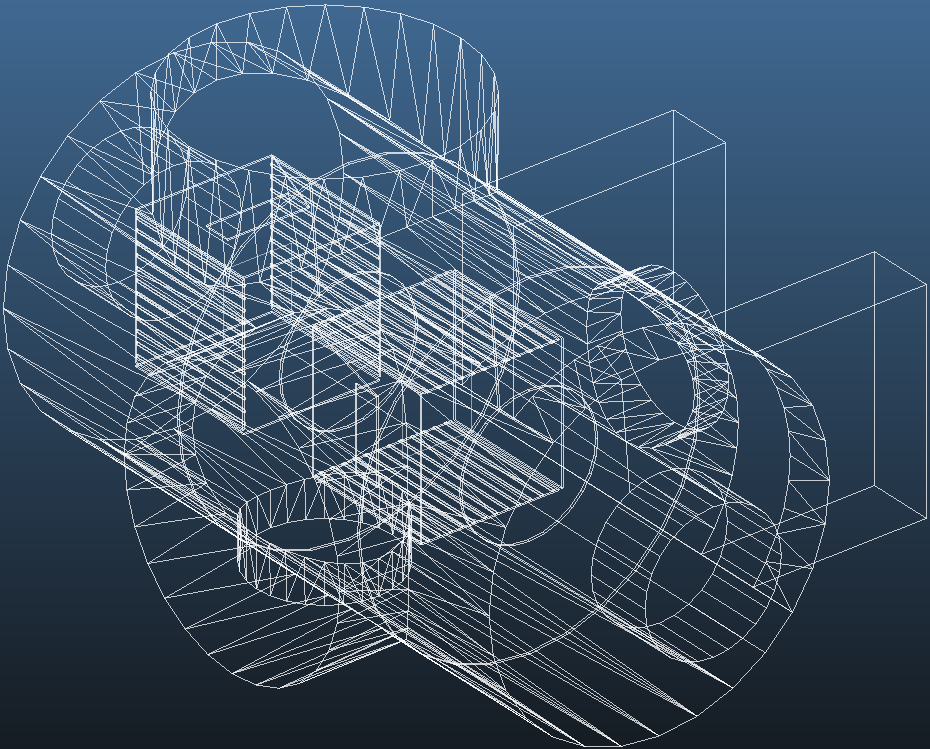
\includegraphics[width=0.5\textwidth]{03_Prototype/figures/fig019_molflow_LWU.png}
  \caption[The LWU geometry implemented in Molflow+]{The LWU geometry implemented in Molflow+.}    
	\label{chap3:molflow_LWU}
\end{wrapfigure}


  A simulation has be done with the Molflow+ software developed at CERN \cite{Kersevan2009}. It simulates the vacuum in a steady state by Monte Carlo methods. The user defines his geometry, the desorption and adsorption rates of each surface. The geometry used is visible in Fig. \ref{chap3:molflow_LWU}. Hence, it does not contain all the structures and surfaces. Two dummy squares facets of $5\,\mathrm{cm}$ are inserted in the center of each \acrshort{ipm}. The pressure profiles are then measured on these facets. We have no information about pumping groups, surface conditions or other vacuum characteristics. Therefore, the simulation is not there to exactly determine the vacuum achievable by our system in the LWU but to verify the uniformity of the pressure profile in both \acrshort{ipm}s.

  Fig. \ref{chap3:profile_pressure} shows results from simulation and fortunately pressures seem uniform in the both IPMs. The pressure is slightly lower in the second IPM because the pumping group is closer. However, this may not afflict the profile measurement.

  \begin{figure}[!h]
	\begin{center}
		\includesvg[width=\textwidth]{03_Prototype/figures/fig020_profile_pressure}
	\end{center}
	\caption[Simulated profile pressure in the center of IPMs.]{Simulated profile pressure in the center of IPMs.}
	\label{chap3:profile_pressure}
\end{figure}



  \section{Profile distortion effects}
  % TODO: Commencer cette partie
  
  \section{Extraction field}
  % TODO: A faire corriger
  The \acrshort{ipm}s can be seen as a parallel plate detector. In an ideal \acrshort{ipm} these plates are infinite sized. The extraction field is then completely oriented in a single direction, normal to the detection plane. So the projection of the profile is perfect on this plane. In reality, the plates can not be considered infinite sized because the distance between the two electrodes is equal to the gap size between them. In these conditions the field is no more uniform for several reasons including:
  \begin{itemize}
    \item The effects induced by the sides of the cage are no longer negligible. Uniformity is strongly influenced by the peak effects of the plates.
    \item The geometry of the vacuum chamber has also some influences on the field uniformity. Indeed the vacuum chamber is considered to be at ground. Walls close to the \acrshort{ipm}s will change the electric field lines inside the \acrshort{ipm}s.
    \item The way to create the field with high voltage (\acrshort{hv}) power supplies. We will see later that some readouts can only work in certain configurations of high voltages.
    \item The cross-interaction between two IPMs close by.
  \end{itemize}
  The non-uniformity of the electric field is very problematic because it prevents the correct measurement of the beam profile. It also determines the maximum size of the detection area which must be in a zone as uniform as possible. To overcome all these effects, several solutions can be considered:

  \begin{itemize}
    \item By reducing the distance between the two electrodes for a same electrode size. In this case, the \acrshort{ipm}s will tend to a configuration close to the infinite parallel plates assumption. However, the \acrshort{ipm}s should not be on the direct path of the beam or its halo to avoid damage. So, the minimum distance between two plates must be at least equal to the diameter of the beam pipe. In same way, the size of both electrodes can be significantly increase. However, this solution is mainly limited due to mechanical considerations. The whole assembly for one \acrshort{ipm} must sustain on a CF 200 flange. The second limitation concerns possible \acrshort{hv} breakdowns. In very high vacuum a distance of some millimeter is sufficient to isolate several tens of kilovolts. However, the breakdowns are also strongly influenced by the surface states of the electrodes, the composition of the vacuum and the presence of leakage current \cite{Latham1995}. Hence, we should keep a standoff distance between the electrode and the vacuum vessel.
    \item The field uniformity can be improved by the use of field correctors or field degraders. This is done by placing conductors on the side. Each corrector is set at a certain potential in order to constraint the field. This solution is easy to implement, compact, and very versatile because independent of the geometry of the \acrshort{ipm}. However, it requires a large number of \acrshort{hv} feedthroughs or the use of resistors in vacuum. The longitudinal field can be corrected in the same way with as long as the degraders do not encroach on the beam path as explained in the previous paragraph.
    \item To protect against the \acrshort{ipm} cross-interaction, one can put grounded conductors between the two \acrshort{ipm}s.
    \item The geometry of \acrshort{hv} electrodes. For example, a curved geometry with reinforcements on the edges it is possible to correct the field transversely and longitudinally \cite{Bartkoski2014}. Hence, there is no more need of field correctors. On the other hand, the electrode is generally larger electrode and optimized for a precise configuration.
    \item Lastly, software corrections may be a solution to correct the non uniformities. However, the non-uniformity of extraction field is not the only phenomenon responsible of the profile distortions as explained just before. It is therefore extremely difficult to implement and requires a perfect map of the extraction field to decouple it from other phenomena. Physical corrections are then much simpler to implement.
  \end{itemize}


  \subsection{Maxwell equations at steady state}
  % TODO: Commencer cette partie
  Electric and magnetic fields are perfectly described by the Maxwell's equations. We suppose to be in a vacuum, so the Maxwell's equations can be written as:
  \begin{alignat*}{3}
    \overrightarrow{\nabla} \cdot \overrightarrow{E} &= \frac{\rho}{\epsilon_{0}}\quad &&\text{(Maxwell-Gauss's Law)}\\
     \overrightarrow{\nabla} \times \overrightarrow{E} &= - \frac{\partial \overrightarrow{B}}{\partial t}\quad &&\text{(Maxwell-Faraday's Law)}\\
     \overrightarrow{\nabla} \cdot \overrightarrow{B} &= 0\quad &&\text{(Maxwell-Thomson's Law)}\\
     \overrightarrow{\nabla} \times \overrightarrow{B} &= \overrightarrow{J} + \frac{\partial \overrightarrow{E}}{\partial t}\quad &&\text{(Maxwell-Ampère's Law)}
  \end{alignat*}

  The time derivatives cancel each other, when the field variations over time are negligible compare to the studied phenomena. So, the coupling effects between the electric and the magnetic fields disappear. Therefore, the electrostatic field depends only on the Gaus’s law. In electrostatic, it is quite convenient to introduce the electric potential:
  \begin{equation}
    \vec{E} = - \vec{\nabla}V
  \end{equation}

  \subsection{Solving Poisson's equation}
  The electric potential follows a Poisson's equation:
  \begin{align}
    &\Delta V = \vec{\nabla}^{2}V = -\frac{\rho}{\epsilon_{0}}\\
    &\Delta v = f
  \end{align}
  
  The solution of this equation can be found analytically. These methods mainly rely on the use of complex numbers or Laplace transforms. However, when the size of the problem increases the solution becomes harder to compute, and solving the Poisson's equation on complicated domains is almost impossible. The numerical methods allow to approximate the solutions of partial differential equations (\acrshort{pde}) on complex domains. There are many schemes to solve numerically \acrshort{pde}. In this section we will briefly present three methods that are used very often. It is important to understand how they work and know their limitations or pitfalls. In numerical schemes, the domain is discretized in a finite set of points. Then, the solution is approximated at each point with respect to initial and/or boundary conditions. To solve a problem, it must be well posed: the problem must admit a single unique solution that depends continuously on the variables and conditions \cite{Hadamard1902}. It turns out that the Poisson's equation is a well-posed problem if a Dirichlet condition is applied.

  Finite Difference Method (FDM) is a popular way to solve numerically the Poisson’s equation. In FDM, the domain is discretized regularly with a step h. The Taylor's theorem allows to approximate the value of a function by a polynomial equation that depends on its derivatives nearby:  
  \begin{align}
     & v(x+h) = v(x)+hv^{\prime}(x)
    +\frac{h^2}{2}v^{\prime\prime}(x)+\frac{h^3}{6}v^{\prime\prime\prime}(x) + O(h^{4}) \\
     & v(x-h) = v(x)-hv^{\prime}(x)
    +\frac{h^2}{2}v^{\prime\prime}(x)-\frac{h^3}{6}v^{\prime\prime\prime}(x) + O(h^{4})
  \end{align}

  From these formulas, the second derivative can be expressed and in case of a two-dimensional domain it is written as follows:

  \begin{equation}
    \begin{split}
      h^{2}v^{\prime\prime}(x,y)=&v(x+h,y) + v(x-h,y) \\
      + &v(x,y+h) + v(x,y-h) \\
      - 4&v(x)+ O(h^{2})
    \end{split}
  \end{equation}

	Each point of the domain can be expressed according to its neighbor. Then, it is possible to write a set of linear equations in matrix form by choosing wisely the indexing order. For example, when the domain is decomposed line by line, one can obtain the same system of equations repeated for each inner line \footnote{The first and last lines have a slightly different set of equations.}. 

  \begin{equation}
    Id \cdot v_{u} + A \cdot v_{c} + Id \cdot v_{d} = D   
  \end{equation}
  Where $ A =
    \begin{pmatrix}
    -4     & 1      & 0      & \cdots \\
    1      & -4     & 1      & \cdots \\
    0      & 1      & -4     & \cdots \\
    \vdots & \vdots & \vdots & \ddots
    \end{pmatrix} $ is square matrix of FDM schemes, $v$ is the unknown value vector and $D$ is vector of Dirichlet values. Then, the global matrix is assembled by combining the sub-matrices for each line.

  \begin{equation}
    \begin{bmatrix}
      A      & Id     & 0      & \cdots \\
      Id     & A      & Id     & \cdots \\
      0      & Id     & A      & \cdots \\
      \vdots & \vdots & \vdots & \ddots
    \end{bmatrix}
    \cdot
    \begin{bmatrix}
      v \\
      v \\
      v \\
      \cdots
    \end{bmatrix}
    =
    \begin{bmatrix}
      D \\
      D \\
      D \\
      \cdots
    \end{bmatrix}
  \end{equation}

  On can see that the problem is solved by inverting the A matrix. This matrix is very sparse and can be inverted with iterative methods rather than a direct inversion. FDM is straightforward and allows to quickly solve Poisson’s equation on a linear structured mesh. For example, It is very useful for calculating an electric field generated by a charge density. However, FDM cannot be used when the geometry becomes too complex.

  The Finite Element Method (FEM) is more suitable for solving PDE on complex domains. The FEM uses the weak formulation of the Poisson’s equation. By introducing a test function, this weak form can be written easily thanks to a integration by parts:
  \begin{align}
    \int_{\Omega}^{} \varphi \Delta v d\Omega                                                                             & = \int_{\Omega}^{} \varphi f d\Omega \\
    \int_{\Omega}^{} \vec{\nabla} \varphi \cdot \vec{\nabla} v d\Omega - \int_{d\Omega}^{} \varphi \vec{\nabla} v \cdot n d\Sigma & = \int_{\Omega}^{} \varphi f d\Omega                                                      \\
    \int_{\Omega}^{} \vec{\nabla} \varphi \cdot \vec{\nabla} v d\Omega & = \int_{\Omega}^{} \varphi f d\Omega + \int_{d\Omega}^{} \varphi \vec{\nabla} v \cdot n d\Sigma
  \end{align}

  One can see that the Laplacian disappeared from the formulation. An approximation of v is done in the reduced domain by the mean of low order polynomial functions. Again, a finite system of linear equations can be written, and the problem is solved by inverting the matrix. The correct choice of test functions and the way to index elements lead to very sparse matrix which can be inverted easily. Unlike the FDM, the solution is approximated on the whole reduced domain and not locally. FEM supports complex meshes as long as they are continuous and solves all kinds of PDEs that may be much more complex than the Poisson’s equation.

  With FEM, the whole domain is fully discretized. Whereas according to Green's theorem [Introduire fonction Green?] ... In the case of electrostatic, it is possible to use the Boundary Element Method. With the BEM, the Poisson’s equation is first solved on boundaries. Then, the electric potential can be evaluated at any point in the domain from the contributions of all boundaries. The discretization is also performed only on the boundaries and not on the entire geometry. So, the dimension of the problem is reduced and the matrix to be reversed is then much smaller. On the other hand, the matrix is ​​no longer sparse.

  Most of the commercial simulation softwares rely on FEM or BEM \cite{cststudio2018,ansys2018,couloumb2018}. We have used mainly COMSOL software for the simulations of extraction field.

  \subsection{COMSOL}
  COMSOL is proprietary all-in-one multi-physics simulation software able to solve various problems from structural mechanical analysis to optical raytracing \cite{comsol2018}. We use COMSOL with the AC/DC module to simulate the static electric field in the \acrshort{ipm} box \cite{comsolacdc2018}. COMSOL allows to quickly define, simulate and post process physical model. The typical workflow is divided in three main steps.

  The first step is to implement the detector geometry into COMSOL. The software includes basic \acrshort{cad} features that allows to quickly create two or tridimensional geometries. The users can directly import a mesh from file generated by external \acrshort{cad} tools. However, importing from \acrshort{cad} often increases the model complexity and so the simulation time and it is much faster to directly implement the geometry with COMSOL.  In our case, only the inner shape of the vacuum chamber and the \acrshort{ipm}s must be defined. All other conductive bodies that enclose the vacuum are not relevant for an electrostatic simulation. Therefore, the geometry can be simplified. Fig. \ref{chap3:COMSOL_LWU} shows, on the left, a 3D drawing of the \acrshort{ess} vacuum vessel with the two \acrshort{ipm}s within. And on the right, an example of the simplified geometry implemented in COMSOL.

  \begin{figure}[ht]
	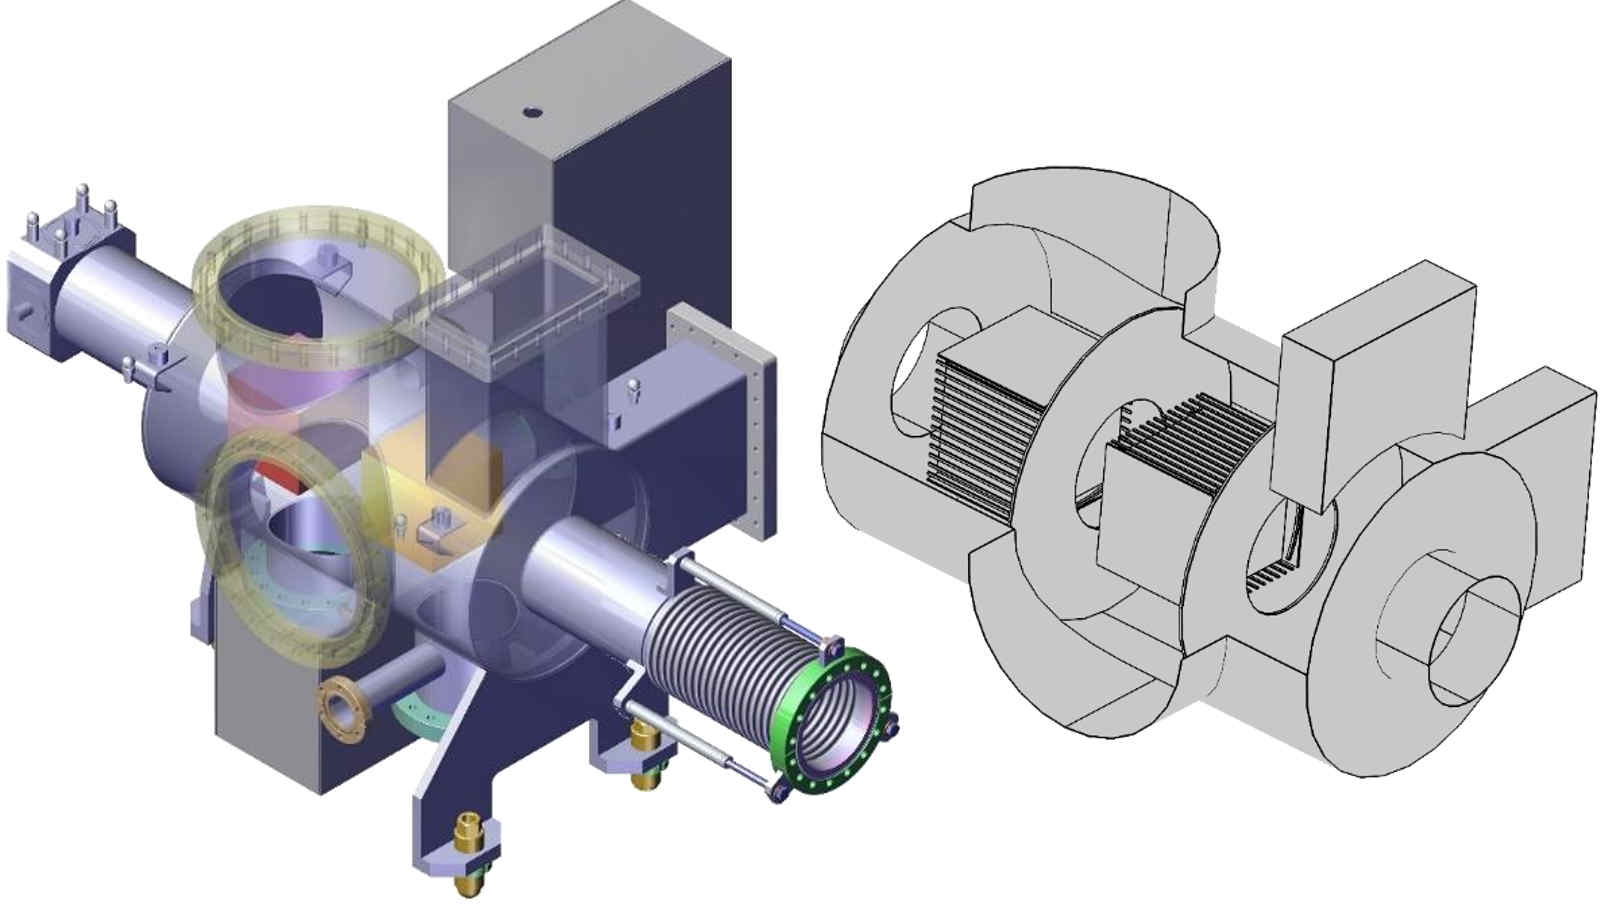
\includegraphics[width=\textwidth]{03_Prototype/figures/fig003_COMSOL_LWU.jpeg}
	\caption[A drawing of LWU (left) and its implementation in COMSOL (right)]{A drawing of LWU (left) and its implementation in COMSOL (right).}
	\label{chap3:COMSOL_LWU}
\end{figure}


  The next step consists on the discretization of the previous geometry in many Lagrange elements in order to form a mesh. Fig. \ref{chap3:COMSOL_meshing_elements} shows main meshing elements available in COMSOL. For an electrostatic tri-dimensional study, COMSOL uses quadratic tetrahedral elements by default. The meshing algorithm tries to create elements that fit well to geometry. So, if a geometry has small parts then the size of elements will be reduced in these regions. Conversely, mesh cells will become bigger and bigger in coarse regions of the geometry. However, this behavior is not desirable for us. Indeed, in an \acrshort{ipm}, the region of interest has no geometrical variation consequently mesh element are particularly big there. This may lead to inaccurate results. Fortunately, the user can change the characteristics and the nature of the elements in specific region of the defined geometry. We used a tetrahedral mesh apart from the \acrshort{ipm} box where a cubic mesh with high granularity is defined. The meshing step is very memory consuming and a poorly optimized mesh may destroy performance.

  \begin{figure}[ht]
	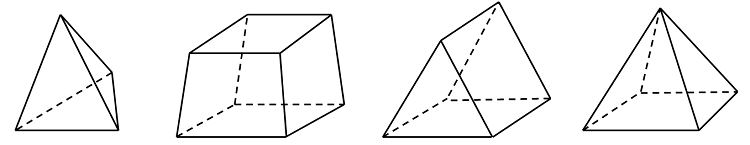
\includegraphics[width=\textwidth]{03_Prototype/figures/fig006_COMSOL_meshing_elements.png}
	\caption[3D Mesh elements included in COMSOL]{Mesh elements included in COMSOL software. From left to right: tetrahedron, hexahedron, prism and pyramid \cite{mesh2013}. COMSOL uses tetrahedral elements by default to mesh a 3D geometry in AC/DC module.}
	\label{chap3:COMSOL_meshing_elements}
\end{figure}


  The last step is to define boundary conditions. COMSOL hides completely the mathematical aspect of the \acrshort{fem}/\acrshort{bem} and directly express the boundary conditions in a physical meaning. In case of the AC/DC module, this means that the user should fix potentials or charge densities on boundaries. A more detailed description of each boundary condition type can be found in the reference manual. COMSOL is able to solve electrostatic problems by means of \acrshort{fem} or \acrshort{bem} since version 5.3a.
  Once solved, the problem can be processed directly in COMSOL. Data can be also exported to an external file in text format (column separated values or VTU format).

  \begin{figure}[!h]
	\begin{subfigure}{.5\textwidth}
		\centering
		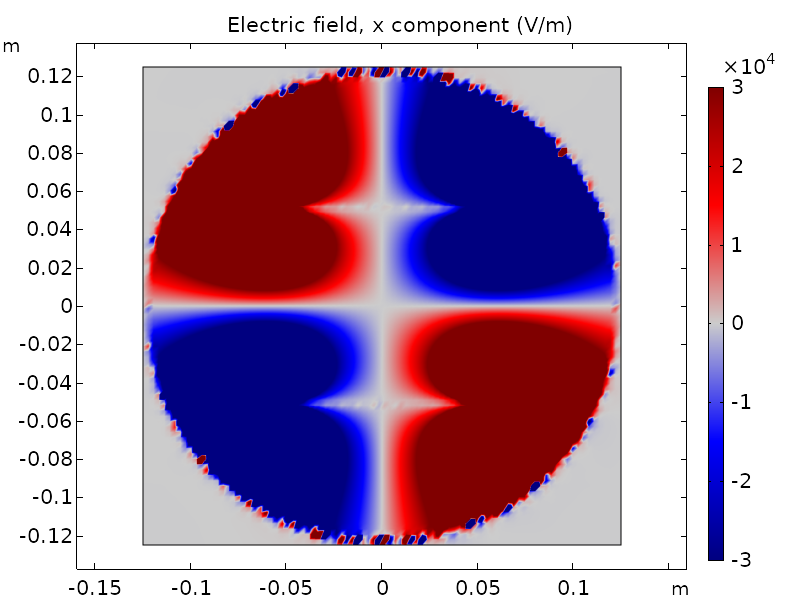
\includegraphics[width=\textwidth]{03_Prototype/figures/fig012_BEMa.png}
		\caption{Configuration 1 solved with BEM.}
		\label{}
	\end{subfigure}\hfill
	\begin{subfigure}{.5\textwidth}
		\centering
		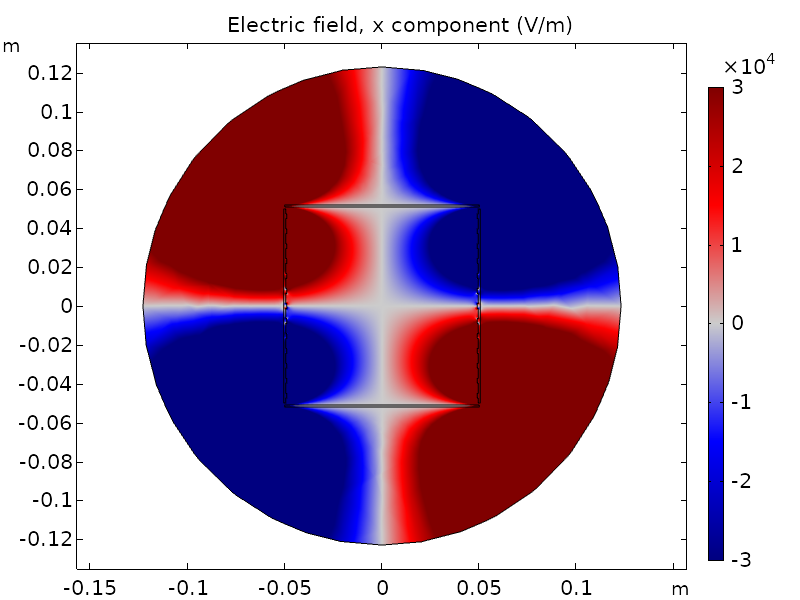
\includegraphics[width=\textwidth]{03_Prototype/figures/fig012_FEMa.png}
		\caption{Configuration 1 solved with FEM.}
		\label{}
	\end{subfigure}
	\vskip\baselineskip
	\begin{subfigure}{.5\textwidth}
		\centering
		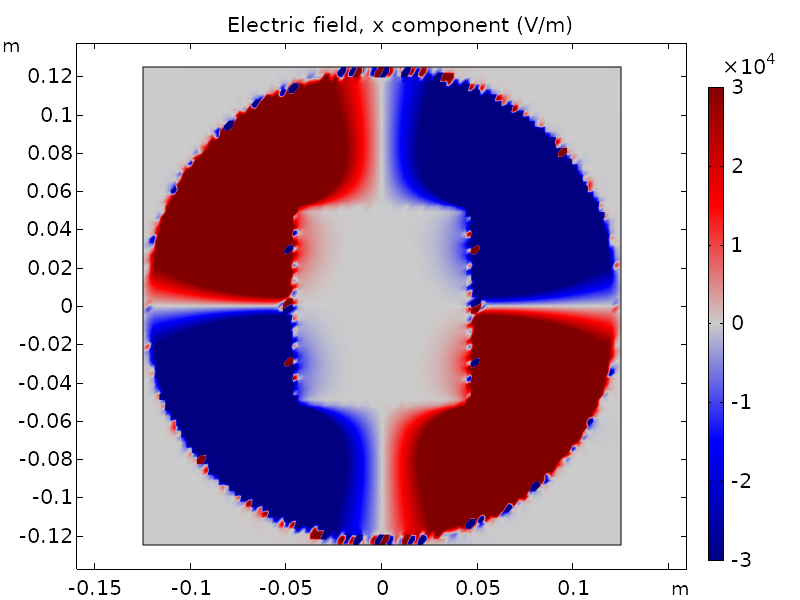
\includegraphics[width=\textwidth]{03_Prototype/figures/fig012_BEMb.png}
		\caption{Configuration 2 solved with BEM.}
		\label{}
	\end{subfigure}\hfill
	\begin{subfigure}{.5\textwidth}
		\centering
		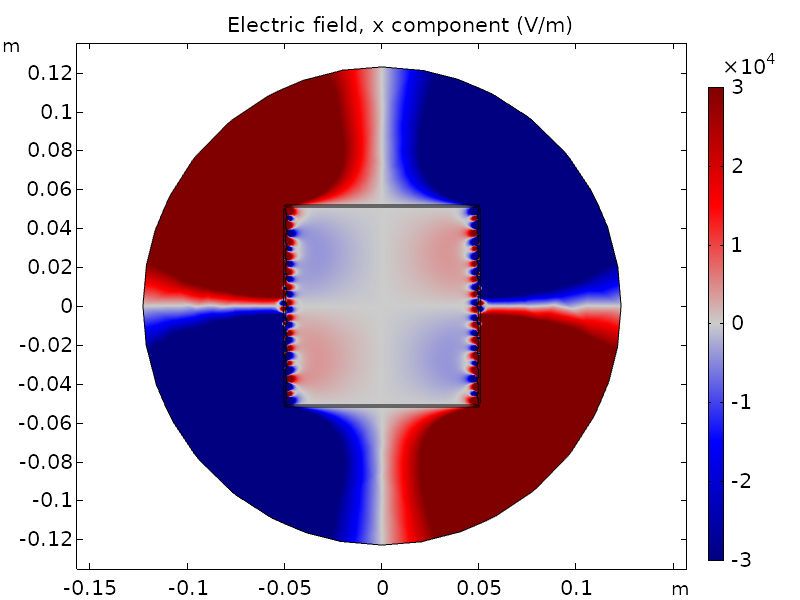
\includegraphics[width=\textwidth]{03_Prototype/figures/fig012_FEMb.png}
		\caption{Configuration 2 solved with FEM.}
		\label{}
	\end{subfigure}
	\caption[Comparison beetwen BEM and FEM for two different IPM configurations]{Comparison beetwen BEM and FEM for two different IPM configurations.}
	\label{chap3:FEMvsBEM}
\end{figure}


  Below is listed the relevant assumptions made in our COMSOL model:
  \begin{itemize}
  \item All conductors and insulators are supposed to be perfect. 
  \item Field correctors and electrodes are thicker than reality since it is not feasible to describe a micrometer deposition layer in a meter scale simulation. 
  \item The resistor chain at the back of field corrector is not implement as well as the connection wires, feedthroughs and connectors. 
  \item The vacuum vessel is supposed to be at the same ground as power supplies, and without any charge on its surface.
  \end{itemize}

  \subsection{Criteria}

  Now, it is necessary to define criteria that quantify the uniformity of the electric field in order to compare several simulations together. In this thesis, we will use mainly:
  \begin{itemize}
    \item Visual approachs (isocolors and streamline) that are sufficient at first to underline the big differences between two models.
    \item A pseudo-statistical criterion
    \item Particle tracking
  \end{itemize}
  In this setion, we will explain briefly the two last criteria.

  For the pseudo-statistical criterion, the whole data set is sliced in the longitudinal direction. In each slice, the quadratic mean of each electric field component is computed in an area at the center of the IPM.
  \begin{equation}
    \vec{E}_{qmean} = \frac{\sum_{i=1}^{N}\sqrt{\vec{E}_{i}^{2}}}{N}
  \end{equation}
  The only pitfall of this method is the size of the area. The mean must be computed on an area that covers at least the beam\footnote{We assume that the beam is centered}. On the other hand, if the area is to big, then the mean value will be biased due to field correctors on each side of the IPMs.
  To choose the area size, we proceed a follows. A charged particle is released at rest in a dummy IPM where the field is perfectly uniform except in a small region. In this region, we add an fully orthogonal component equal to $1\,\mathrm{\%}$ of the main field value. When the particle reaches the readout, the total deviation is recorded. Then the region is shifted and the computation is repeated. Table \ref{chap3:Deviation}tabulates results.

  \begin{table}[ht]
	\centering
	\caption[Example of deviation of the trajectory of a particle in an IPM]
	{Example of deviation of the trajectory of a particle in an IPM. A particle is released in the center of an IPM with a straight field everywhere, but in a certain range a parasitic field component is added and set to $1\,\mathrm{\%}$ of the main field. The 0 coordinate is the IPM center whereas the readout is at \(5 \, \mathrm{cm}\) distance.}
	\label{chap3:Deviation}
	\begin{tabular}{cccccc}
		\toprule
		                               & \multicolumn{5}{c}{Range (\(\mathrm{cm}\))}                                                 \\
		\cmidrule(lr){2-6}
		                               & \([0,1]\)                                   & \([1,2]\) & \([2,3]\) & \([3,4]\) & \([4,5]\) \\
		\midrule
		Deviation (\(\mathrm{\mu m}\)) & \(347\)                                     & \(85\)    & \(42\)    & \(20\)    & \(5.6\)   \\
		\bottomrule
	\end{tabular}
\end{table}

  One can see that the deviation is quite important when the particle has almost no kinetic energy, i.e. when the particle is created.
  At the end of the drift, the particle has much more kinetic energy so it is less affected by field non-uniformities. So, the field must be optimized to be the most uniform in IPM center. The non-uniformities on the IPM sides are less concern.
  So we decided to compute the quadratic mean inside a circle of at least two centimeter radius. However, it is impossible to predict the real effects on the profile since the quadratic mean shadows the direction of the field.

  The tracking algorithm is in theory the most relevant criterion for an IPM. Particles are released and we observe drift in the field cage due to electric and/or magnetic fields, thanks to Lorentz’s force: 
  \begin{equation}
    \vec{F} = m \cdot a = q \cdot (\vec{E}(\vec{r},t) + \vec{v} \times \vec{B}(\vec{r},t))
  \end{equation}
  Initial particle positions are drawn following an ESS pulse shape characteristics in longitudinal and time space. The equation of motion is integrated with a numerical integrator. The value of field at an arbitrary position is interpolated from values computed by COMSOL. These steps are repeated until the particles reach the detection system. The simplest numerical method is probably the Euler integration, written as follow in case of the Lorentz’s force:
  \begin{align}
    & \vec{v}_{i} = \vec{v}_{i-1} + \frac{q}{m}(\vec{E}(\vec{r}_{i-1},t) + \vec{v}_{i-1} \times \vec{B}(\vec{r}_{i-1},t)) \cdot \Delta t \\
    & \vec{r}_{i} = \vec{r}_{i-1} + \vec{v}_{i} \cdot \Delta t
  \end{align}
  This algorithm is straightforward and can be implemented in few lines of code. On the other hand it is first order integrator, therefore the accuracy is not good. Higher orders methods, like Runge-Kutta integrators, provide more accuracy, thus they are very popular integrators for solving various types of ordinary differential equations (ODE). However, all previous methods doesn’t provide good accuracy with the Lorent’s force when a magnetic field is present. The Boris method provides a workaround to this problem \cite{Boris1970}, moreover its algorithm is really straightforward :
  \begin{align}
     & \vec{v}^{-} = \vec{v}_{i} + \frac{q}{m} \frac{\Delta t}{2}\vec{E}\\
     & \vec{v}^{'} = \vec{v}^{-} + \frac{q}{m} \frac{\Delta t}{2}(\vec{v}^{-} \times \vec{B})\\
     & \vec{v}^{+} = \vec{v}^{-} + \frac{\frac{q}{m}\Delta t}{1+(\frac{q}{m} \frac{\Delta t}{2}\vec{E})^{2}}(\vec{v}^{-} \times \vec{B})\\
     & \vec{v}_{i+1} = \vec{v}^{+} + \frac{q}{m} \frac{\Delta t}{2}\vec{E}
  \end{align}
  One can see that the E and B field are separated. This algorithm is almost a standard in particle in cell (PIC) codes because it remains extremely accurate even during long integration time \cite{Qin2013}.
  
  During the tracking, the field is evaluated at each step in order to calculate the new velocity and position. The field values must be interpolated because the original field dataset is composed of discrete values. The mesh is usually not structured with FEMs, therefore the interpolation is not trivial. The interpolation can be done by a nearest neighbor search. The returned values is the same as the one on the closest point with respect to a metric distance. This method is fast and straightforward to implement but leads to massive errors if the mesh is not regular enough. It can be improved by weighting the returned with the distance for several closest points, this is known as Shepard interpolation. However, the accuracy still perfectible. Radial Basis Function (RBF) interpolation is one of the most powerful interpolation method that works on unstructured data [expliquer plus ?]\cite{Wright2003}. We mainly used this method to interpolate our fields during the particle tracking. 

  \begin{figure}[!h]
  \begin{subfigure}{0.5\textwidth}
    \includesvg[width=\textwidth]{03_Prototype/figures/fig017_interpolation1D}
    \caption{}
    \label{}
  \end{subfigure}
  ~
  \begin{subfigure}{0.5\textwidth}
    \includesvg[width=\textwidth]{03_Prototype/figures/fig014_numerical_integration}
    \caption{}
    \label{}
  \end{subfigure}

  \caption[]{}
  \label{chap:}
\end{figure}


  The tracking algorithm has been implemented in an C++ code. All vector operations are performed by the Eigen package and custom code \cite{eigenweb}. Nanoflann library build a kd-tree from field data \cite{blanco2014nanoflann}. It allows to quickly search a set of points inside the whole dataset. The interpolation routine is homemade and relies on previous libraries. The routine implement nearest neighbors and Radial Basis Function interpolations. The numerical integration of positions and velocities are perform by homemade code and Odeint library \cite{Ahnert2011,Mulansky2014}. Particle are tracked in parallel with the Intel TBB library \cite{tbb2019}.
  
  \subsection{IPM polarity}

  In an IPM, the extraction field can be generated with different kinds of high voltage configurations. However, some readouts can not operate at high voltages. In this case, the readout electrode must be at ground level in order to avoid damages on the readout. Hence, the choice of the HV configuration is fully determined by the choice of the readout. In the following, we will consider two configurations:
  \begin{itemize}
    \item Symmetric configuration when the readout can work at high voltage. In this case, the electrode have opposite potential.
    \item Asymmetric configuration when the readout electrode is at ground and the other electrode is at a certain potential.
  \end{itemize}

  The two configurations have been simulated in COMSOL and the results are presented in the Fig. \ref{chap3:asym_sym}. One can see that without any correction the extraction field in symmetric configuration is much more uniform. 
  
  In this configuration (Fig. \ref{chap3:asym_sym_b}), the field focuses the particles in the transverse plane but also in the longitudinal plane. This explains why the particle number on the readout is higher than the expected number. In symmetric, only the transverse plane should be corrected.

  In asymmetric configuration (Fig. \ref{chap3:asym_sym_a}), the field is defocusing in the transverse plane, but also in the  longitudinal one. The projection of the beam will be much broader than expected and many particles are lost during the particle drifts. Therefore, the electric field must be improved in both planes.


  \begin{figure}[!ht]
	\begin{subfigure}{0.5\textwidth}
		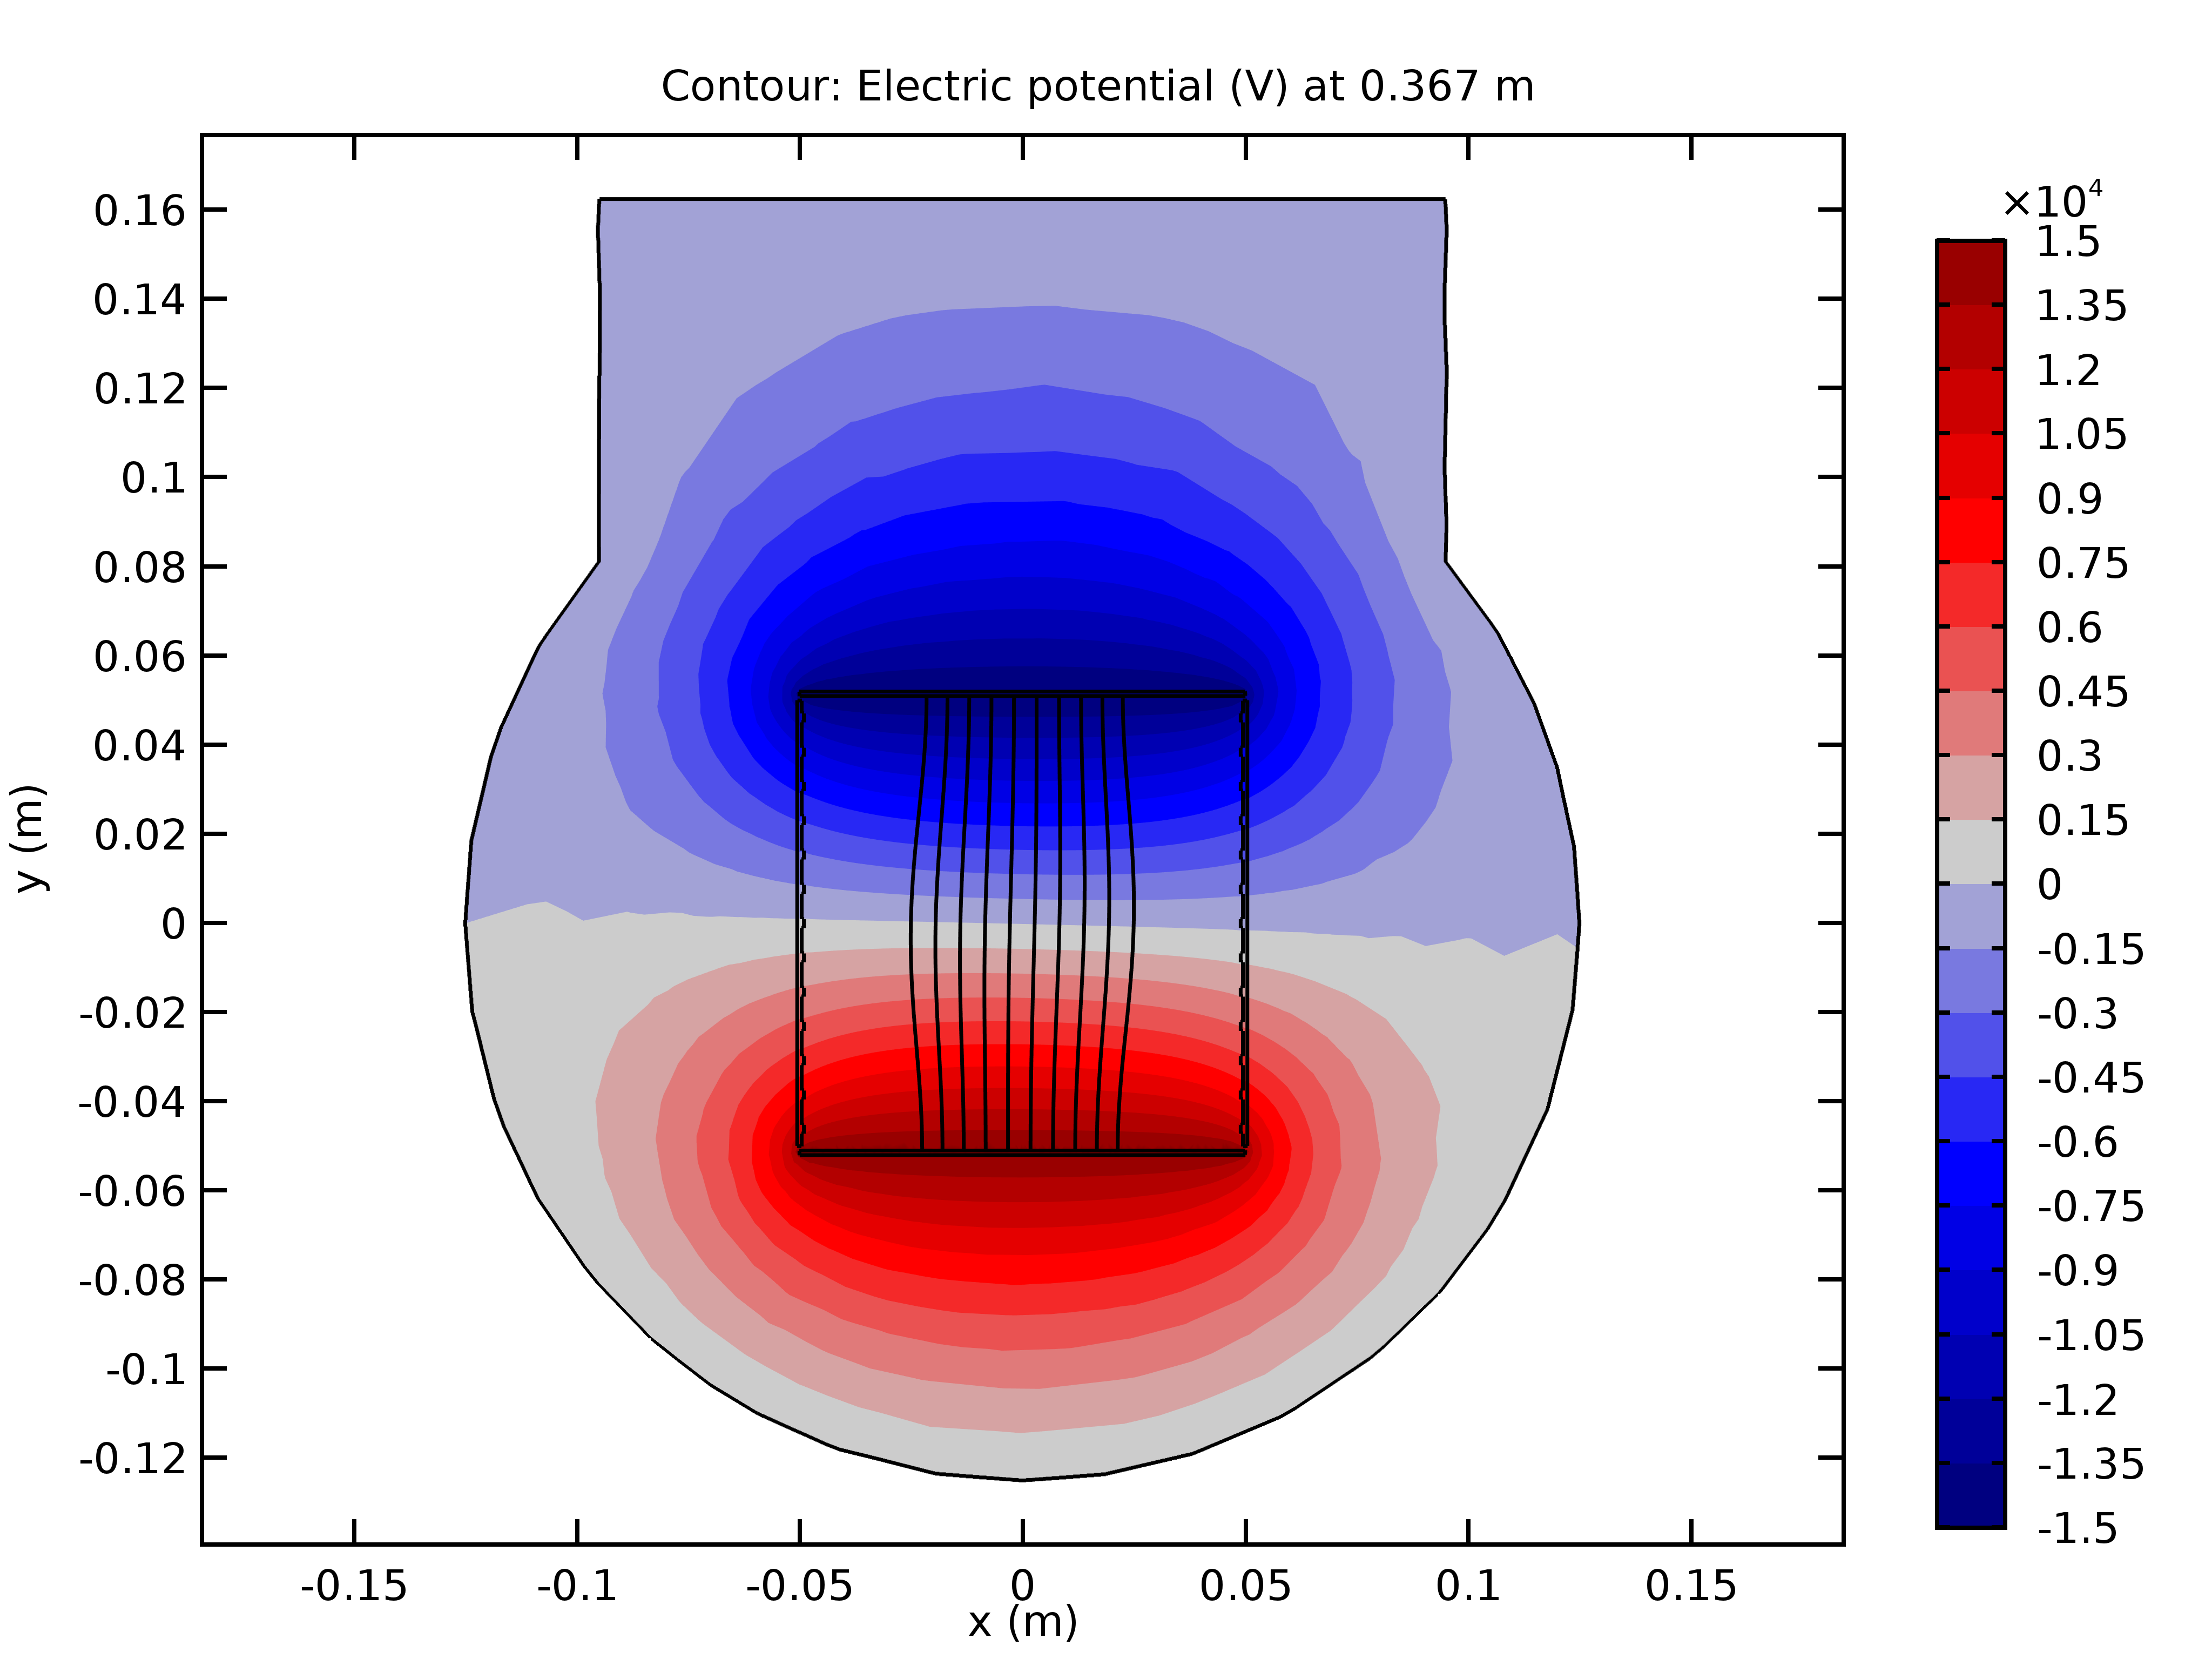
\includegraphics[width=\textwidth]{03_Prototype/figures/fig021_image_asym_sym_b.png}
		\caption{Symmetric configuration.}
		\label{chap3:asym_sym_b}
	\end{subfigure}
	~
	\begin{subfigure}{0.5\textwidth}
		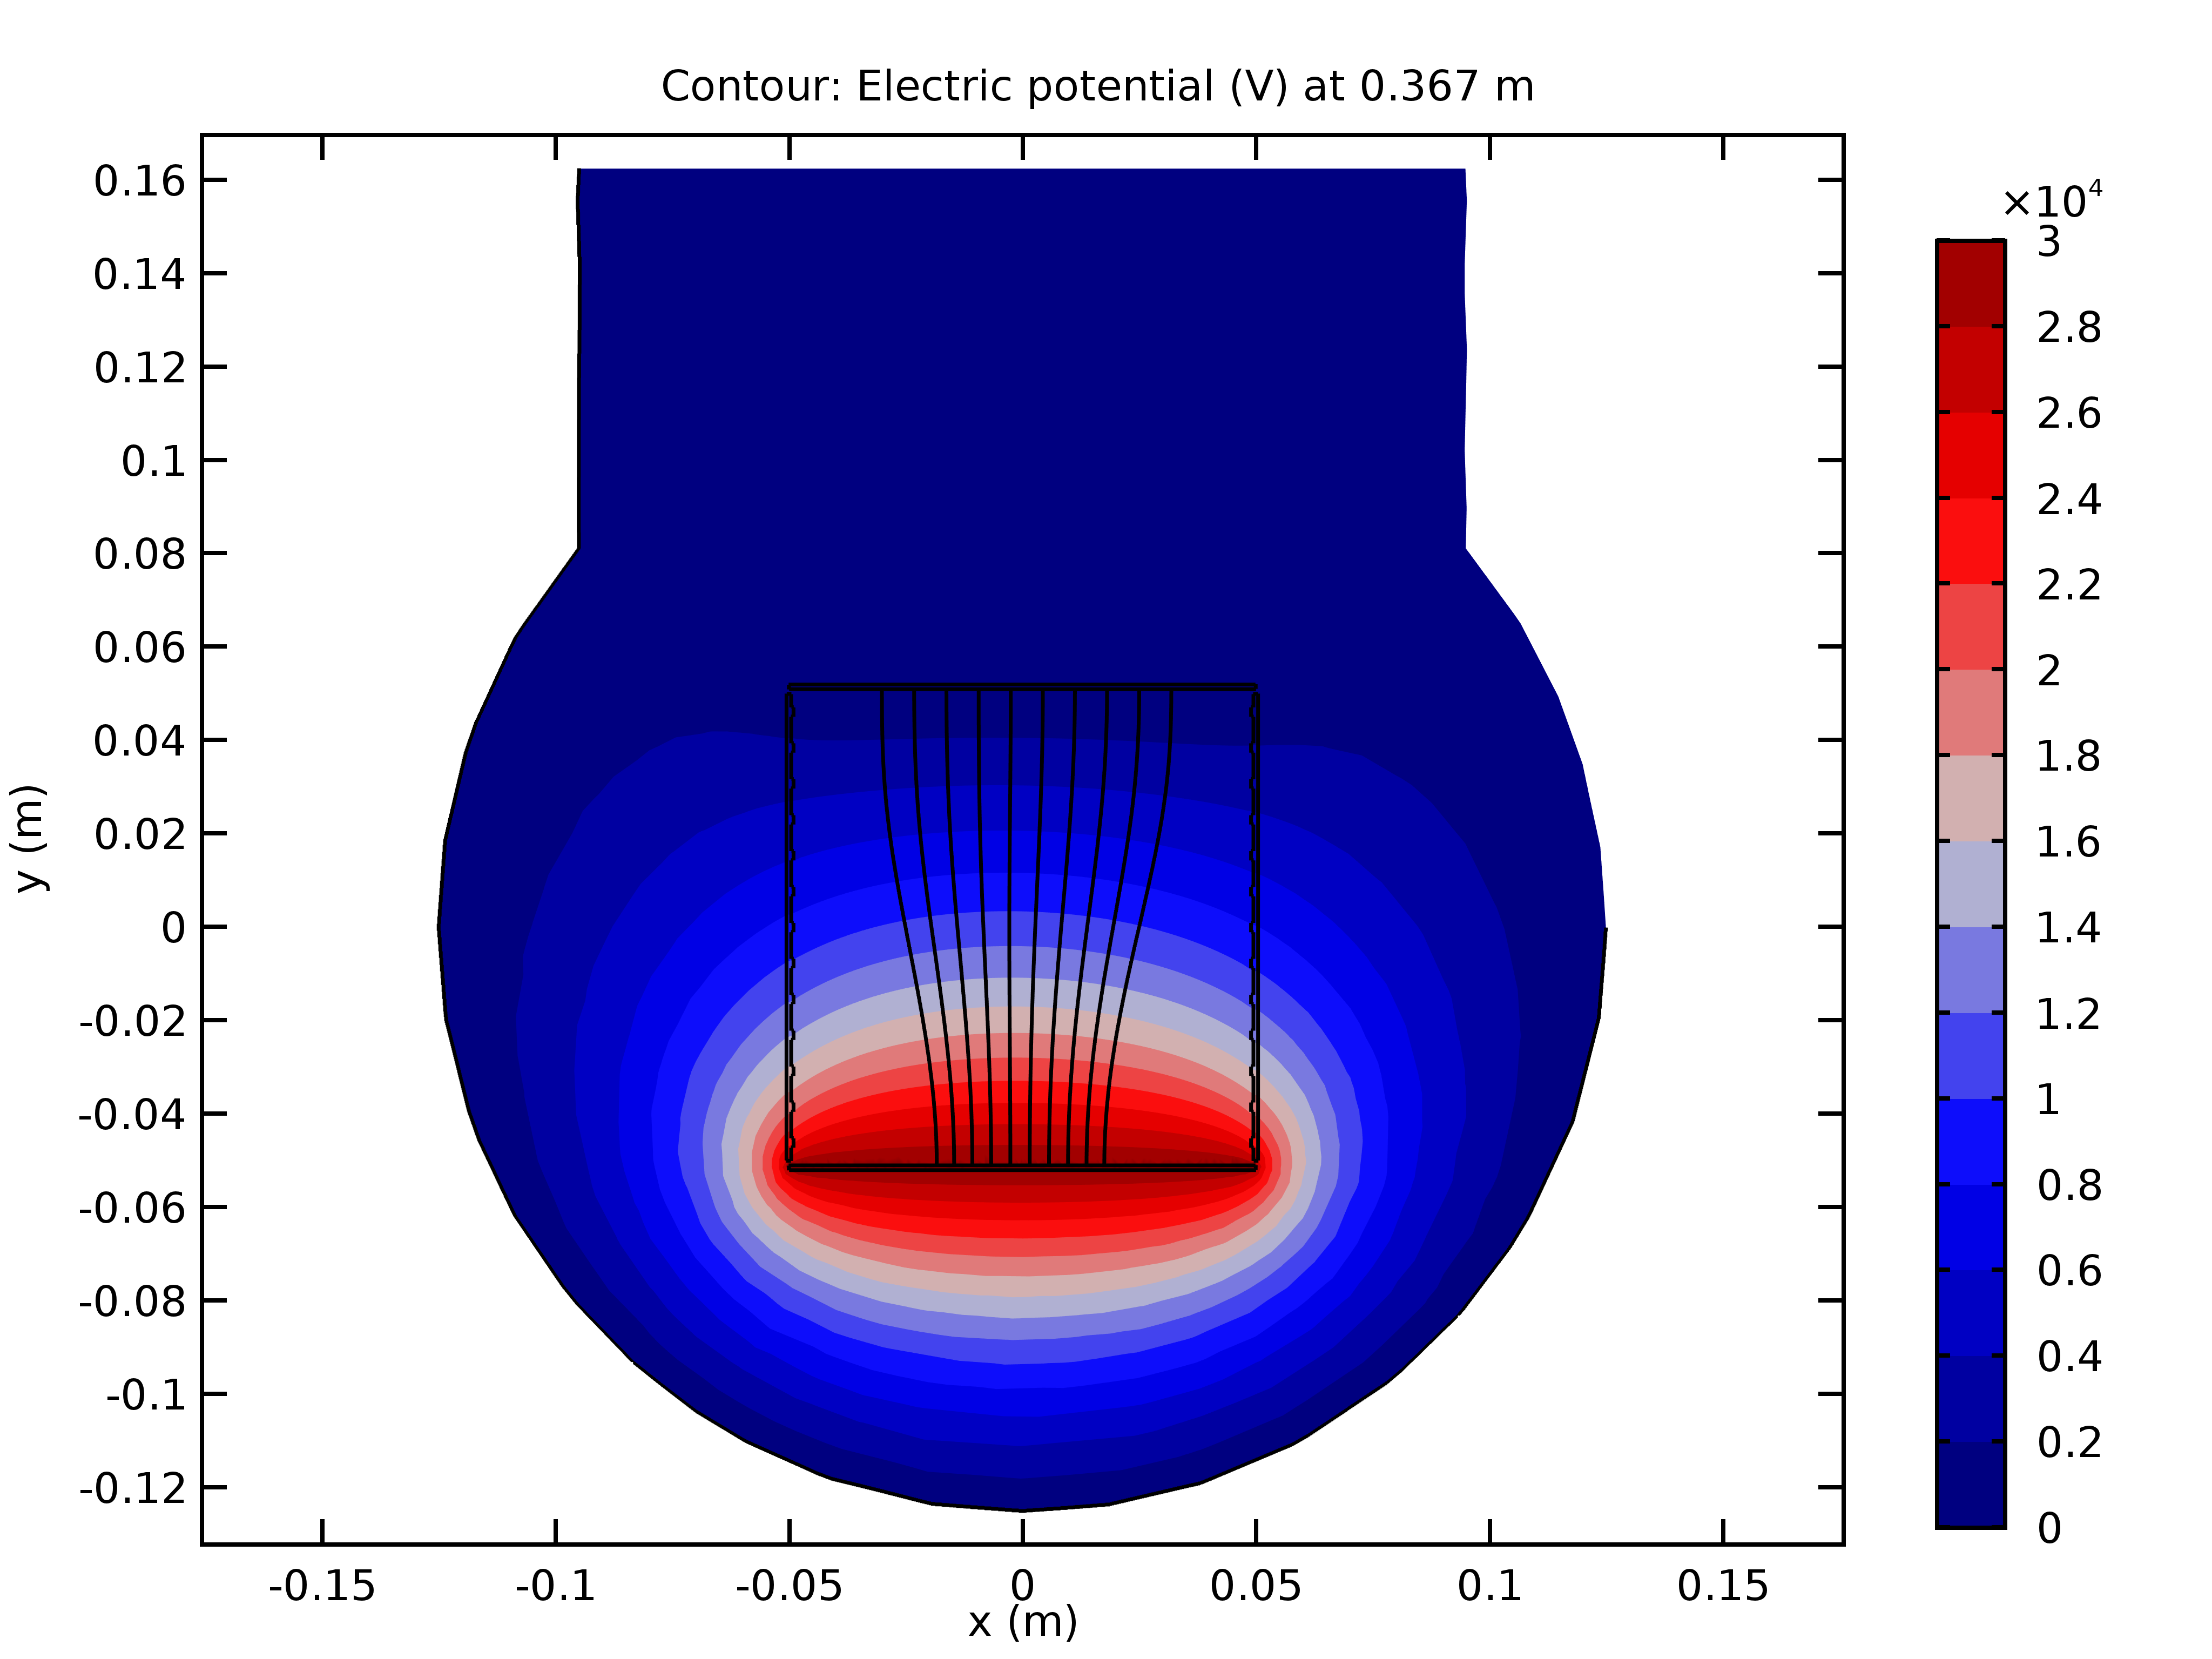
\includegraphics[width=\textwidth]{03_Prototype/figures/fig021_image_asym_sym_a.png}
		\caption{Asymmetric configuration.}
		\label{chap3:asym_sym_a}
	\end{subfigure}
	\caption[Comparison between symmetric and asymmetric configuration]{Comparison between symmetric and asymmetric configuration.}
	\label{chap3:asym_sym}
\end{figure}


  \subsection{Field corrections}
  As explained previously, the electric field will be improved by means of field correctors (also called field degraders) and curved electrodes. The Fig shows the COMSOL an example of IPM that has been simulated. One can see the degraders on each side and the curved electrodes at the top and bottom of each of the IPM.

  %\begin{wrapfigure}{l}{0.3\textwidth}
	\begin{center}
		\begin{tikzpicture}[scale=0.8,transform shape,american voltages]
			\draw (0,0) node[label={above:HV}] {} to [short, *-] (2,0)
			to [R, l_=$R_1$] (2,2)
			to [R, l_=$R_2$, *-] (2,4);
			\draw (0, 9) node[label={above:HV}] {} to [short, *-] (2,9)
			to [R, l_=$R_{N}$] (2,7)
			to [R, l_=$R_{N-1}$, *-] (2,5)
			(2,4.5) node[] {...};
		\end{tikzpicture}
	\end{center}
	\caption[Resistor chain]{Resistor chain.}
	\label{chap3:resistor_chain}
\end{wrapfigure}


  The field correctors will constrain the electric potential at a certain value on the side of the IPM. Thus, the isopotential will be more flat in the IPM, so the field be more uniform. In practice, field degraders are just conductive pieces connected to a voltage source. One can directly connect them to power supplies. This method allows to tune finely the potential on the electrodes. On the other hand, it requires HV feedthroughs for each electric potential. Unfortunately, we cannot do this way since the available space on the IPM flange is restricted. We will use directly the existing high voltages to feed a resistor bridge as shown in Fig.  The potential at each field corrector is simply given by the Ohm law:

  \begin{equation}
    V_{i} = \frac{\sum_{k = 1}^{i} R_{k}}{\sum_{j = 1}^{N} R_{j}}V_{HV}
  \end{equation}

  The method is straightforward to implement but has some drawbacks. The choice of resistor is limited since all resistance values are not available. Thus, all correction possibilities are not possible. The use of resistor in a vacuum is not really recommended since it often require welding. Also, the resistor should should sustain the radiative environment. Moreover, if one of the resistance is damaged the entire bridge is affected.

  \subsection{IPM cross-interaction}

  \begin{figure}[!ht]
  \centering
	\begin{subfigure}{0.8\textwidth}
		\includesvg[width=\textwidth]{03_Prototype/figures/fig022_2IPM_ASYM_NODISK_NODEG_a}
		\caption[]{}
		\label{}
	\end{subfigure}

  \begin{subfigure}{0.8\textwidth}
		\centering
		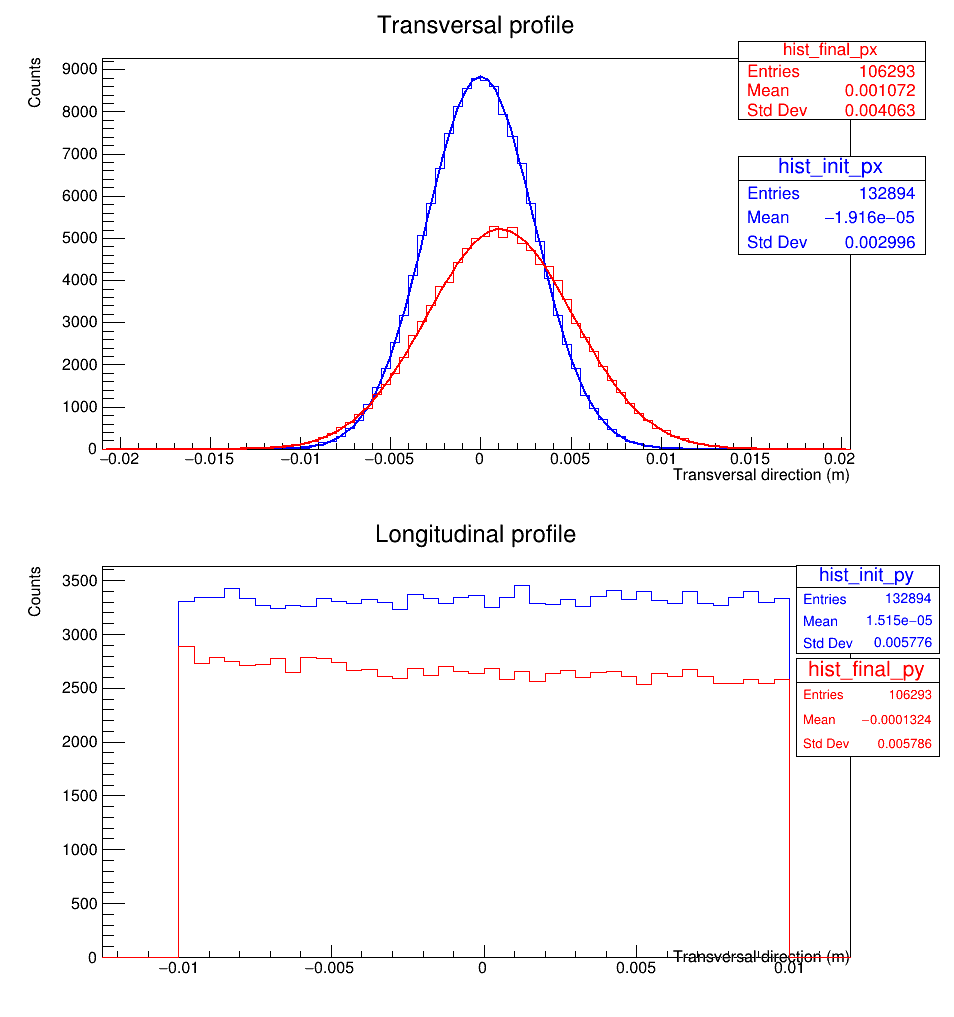
\includegraphics[width=\textwidth]{03_Prototype/figures/fig022_2IPM_ASYM_NODISK_NODEG_b}
		\caption{}
		\label{}
	\end{subfigure}
	\caption[]{}
	\label{chap:}
\end{figure}


  \subsection{Grid}

  \subsection{Summary}

  \section{Initial momentum}
  So far, we assumed that the ions and/or electrons were created without initial velocity ie at rest in a pure electrical field. In this case, electrons and ions give same results and the value of extraction field does not matter. In reality, these particles have a non-negligible initial speed and may be affected by parasitic electromagnetic fields. This can greatly affect the profile, thus the extraction field must be increased in order to minimize the distortion. In the following sections, we will try quantify these effects to determine the nominal value of the extraction field.

  \subsection{Thermal distribution}
  A first approximation of the initial speed of ions can be done thanks to the distribution of Maxwell-Boltzmann. The distribution of the speeds with respect to the particle mass and the temperature is given by the following equation:

  \begin{equation}
    F(\boldsymbol{v}) = \left(\frac{m_{part}}{2 \pi k_{b} T}\right)^{\frac{3}{2}}\exp\left(-\frac{m_{part}\boldsymbol{v}^{2}}{2 k_{b} T}\right)
  \end{equation}
  Where, $k_{b}$ is Boltzmann constant , $T$ the temperature, $\boldsymbol{v}$ is the speed vector of the considered particle and $m_{part}$ its mass.

  % \begin{wrapfigure}{r}{0.5\textwidth}
% 	\includesvg[width=0.5\textwidth]{03_Prototype/figures/fig013_maxwell_gas2}
% 	\caption[Maxwell-Boltzmann distribution for some species of ESS residual gas]{Maxwell-Boltzmann distribution for some species of ESS residual gas.}
% 	\label{chap3:maxwell_gas}
% \end{wrapfigure}
\begin{figure}[!ht]
	\centering
	\includesvg[width=0.7\textwidth]{03_Prototype/figures/fig013_maxwell_gas2}
	\caption[Maxwell-Boltzmann distribution for some species of ESS residual gas]{Maxwell-Boltzmann distribution for some species of ESS residual gas.}
	\label{chap3:maxwell_gas}
\end{figure}

  \subsection{Ionization energy distribution}
  \section{Space charge effect}
  \subsection{Electromagnetic field due to Lorentz boost}
  \subsection{ESS/CEA Space Charge algorithm}
  \subsection{Comparison}
  \section{Readout simulations}
  \subsection{Interaction of particles with low energies}
  \begin{figure}[!h]
	\begin{subfigure}[t]{.5\textwidth}
		\centering
		\includesvg[width=\textwidth]{03_Prototype/figures/fig004_ion_si_deposit}
		\caption[Energy deposition in a silicon layer for various ions]{Energy deposition in a silicon layer for various ions.}
		\label{chap3:ion_si_deposit}
	\end{subfigure}
	~
	\begin{subfigure}[t]{.5\textwidth}
		\centering
		\includesvg[width=\textwidth]{03_Prototype/figures/fig005_electron_si_deposit}
		\caption[Energy deposition in a silicon layer for electrons]{Energy deposition in a silicon layer for electrons.}
		\label{chap3:electron_si_deposit}
	\end{subfigure}
	\caption[Energy deposition in a silicon layer for ions and electron at low kinetic energyies]{Energy deposition in a silicon layer for ions and electron at low kinetic energyies.}
	\label{chap3:si_deposit}
\end{figure}

  \subsection{Ramo-Shockley theorem}
  \cite[]{Ramo_1939}\cite[]{Shockley_1938}\cite[]{Cavalleri1971}\cite[]{Jen1941}
  \subsection{Strips based detection}
  \subsection{Semiconductor based detection}
  \subsection{MCP based detection}

  A MicroChannel Plate (MCP) generates electrons from incident particles. 
  It can be seen as a glass lead plate drilled with micro-metric tilted holes. 
  A specific coating is applied on its input surface to increase secondary emissions. When a particle hits the MCP hole entrance then secondary electrons are emitted. Due to difference of potential, secondaries are drawn towards the channel output and strike hole walls again, creating more and more electrons. Then, electrons are collected on a detection plane that can be a single electrode, multiple electrodes or a phosphorus screen depending on the requirements (sensitivity, spatial and time resolution). Figure \ref{fig:MCPoutline} presents some schematic representations of how an MCP works.

	\begin{figure}[!ht]
	\begin{subfigure}[t]{0.5\textwidth}
		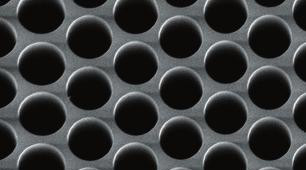
\includegraphics[width=\textwidth]{03_Prototype/figures/fig030_MCPoutline_b2.jpeg}
		\caption[SEM picture of MCP holes]{SEM picture of MCP holes \cite{HamamatsuMCP}.}
		\label{chap3:MCPholes}
	\end{subfigure}
	~
	\begin{subfigure}[t]{0.5\textwidth}
		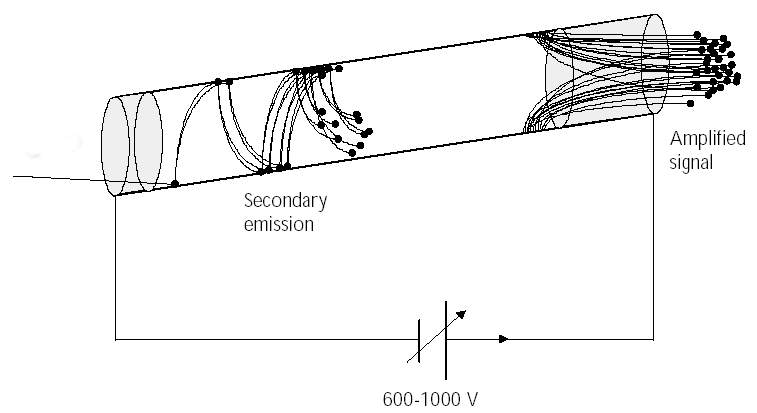
\includegraphics[width=\textwidth]{03_Prototype/figures/fig030_MCPoutline_a.png}
		\caption{Description of how an MCP amplifies incident particle.}
		\label{chap3:MCPchannel}
	\end{subfigure}
	\caption[Schematic views of how a MCP works]{Schematic views of how a MCP works.}
	\label{chap3:MCPoutline}
\end{figure}


  Gain or multiplication factor for a single MCP is about $10^{2}$ to $10^{4}$ depending on the $V_{MCP}$ voltage, usually from 600 to 1000 V. MCP can be stacked to increase the gain to $10^{6}$ or even more. Typical configurations are single stage, chevron stack (double stages) or Z stack (triple stages).

  Unfortunately MCPs have some drawbacks. First one is the lifetime, indeed the coating is damaged by the incident particles thus the gain is not stable and decreases over the time. Second disadvantage is the MCP gain limitation due to saturation mode. If the incident particle flux is too high then holes may be saturated, and they cannot amplify anymore. When it happens to a channel then it takes some times to recover.

  \section{Summary}
  \label{ch3:Summary}
  [Information: textwidth in cm: \printinunitsof{cm}\prntlen{\textwidth}]

  \begin{figure}[!ht]
	\begin{subfigure}[t]{1.\textwidth}
		\includegraphics[width=\textwidth]{example-image-a}
		\caption[]{}
		\label{}
	\end{subfigure}

	\begin{subfigure}[t]{1.\textwidth}
		\centering
		\includegraphics[width=\textwidth]{example-image-a}
		\caption{}
		\label{}
	\end{subfigure}
	\caption[]{}
	\label{chap:}
\end{figure}

  \begin{figure}[!ht]
	\begin{subfigure}[t]{0.5\textwidth}
		\includegraphics[width=\textwidth]{example-image-a}
		\caption{}
		\label{}
	\end{subfigure}
	~
	\begin{subfigure}[t]{0.5\textwidth}
		\includegraphics[width=\textwidth]{example-image-a}
		\caption{}
		\label{}
	\end{subfigure}
	\caption[]{}
	\label{chap:}
\end{figure}

  \begin{figure}[!ht]
	\begin{center}
		\begin{subfigure}{.5\textwidth}
			\includegraphics[width=\textwidth]{example-image-a}
			\caption{}
			\label{}
		\end{subfigure}
	\end{center}

	\begin{subfigure}{0.5\textwidth}
		\includegraphics[width=\textwidth]{example-image-a}
		\caption{}
		\label{}
	\end{subfigure}
	~
	\begin{subfigure}{0.5\textwidth}
		\includegraphics[width=\textwidth]{example-image-a}
		\caption{}
		\label{}
	\end{subfigure}
	\caption[]{}
	\label{chap:}
\end{figure}

  \begin{figure}[!th]
	\begin{subfigure}[t]{.5\textwidth}
		\includegraphics[width=\textwidth]{example-image-a}
		\caption{}
		\label{}
	\end{subfigure}
	~
	\begin{subfigure}[t]{.5\textwidth}
		\centering
		\includegraphics[width=\textwidth]{example-image-a}
		\caption{}
		\label{}
	\end{subfigure}

	\begin{subfigure}[t]{.5\textwidth}
		\centering
		\includegraphics[width=\textwidth]{example-image-a}
		\caption{}
		\label{}
	\end{subfigure}
	~
	\begin{subfigure}[t]{.5\textwidth}
		\centering
		\includegraphics[width=\textwidth]{example-image-a}
		\caption{}
		\label{}
	\end{subfigure}
	\caption[]{}
	\label{chap:}
\end{figure}


  \cleardoublepage
  \section*{Bibliography}
  \addcontentsline{toc}{section}{Bibliography}
  \label{ch3:bib}
  \printbibliography[heading=subbibliography]

\end{refsection}